% Options for packages loaded elsewhere
\PassOptionsToPackage{unicode}{hyperref}
\PassOptionsToPackage{hyphens}{url}
\PassOptionsToPackage{dvipsnames,svgnames,x11names}{xcolor}
%
\documentclass[
  letterpaper,
  DIV=11,
  numbers=noendperiod]{scrreprt}

\usepackage{amsmath,amssymb}
\usepackage{iftex}
\ifPDFTeX
  \usepackage[T1]{fontenc}
  \usepackage[utf8]{inputenc}
  \usepackage{textcomp} % provide euro and other symbols
\else % if luatex or xetex
  \usepackage{unicode-math}
  \defaultfontfeatures{Scale=MatchLowercase}
  \defaultfontfeatures[\rmfamily]{Ligatures=TeX,Scale=1}
\fi
\usepackage{lmodern}
\ifPDFTeX\else  
    % xetex/luatex font selection
\fi
% Use upquote if available, for straight quotes in verbatim environments
\IfFileExists{upquote.sty}{\usepackage{upquote}}{}
\IfFileExists{microtype.sty}{% use microtype if available
  \usepackage[]{microtype}
  \UseMicrotypeSet[protrusion]{basicmath} % disable protrusion for tt fonts
}{}
\makeatletter
\@ifundefined{KOMAClassName}{% if non-KOMA class
  \IfFileExists{parskip.sty}{%
    \usepackage{parskip}
  }{% else
    \setlength{\parindent}{0pt}
    \setlength{\parskip}{6pt plus 2pt minus 1pt}}
}{% if KOMA class
  \KOMAoptions{parskip=half}}
\makeatother
\usepackage{xcolor}
\setlength{\emergencystretch}{3em} % prevent overfull lines
\setcounter{secnumdepth}{5}
% Make \paragraph and \subparagraph free-standing
\makeatletter
\ifx\paragraph\undefined\else
  \let\oldparagraph\paragraph
  \renewcommand{\paragraph}{
    \@ifstar
      \xxxParagraphStar
      \xxxParagraphNoStar
  }
  \newcommand{\xxxParagraphStar}[1]{\oldparagraph*{#1}\mbox{}}
  \newcommand{\xxxParagraphNoStar}[1]{\oldparagraph{#1}\mbox{}}
\fi
\ifx\subparagraph\undefined\else
  \let\oldsubparagraph\subparagraph
  \renewcommand{\subparagraph}{
    \@ifstar
      \xxxSubParagraphStar
      \xxxSubParagraphNoStar
  }
  \newcommand{\xxxSubParagraphStar}[1]{\oldsubparagraph*{#1}\mbox{}}
  \newcommand{\xxxSubParagraphNoStar}[1]{\oldsubparagraph{#1}\mbox{}}
\fi
\makeatother

\usepackage{color}
\usepackage{fancyvrb}
\newcommand{\VerbBar}{|}
\newcommand{\VERB}{\Verb[commandchars=\\\{\}]}
\DefineVerbatimEnvironment{Highlighting}{Verbatim}{commandchars=\\\{\}}
% Add ',fontsize=\small' for more characters per line
\usepackage{framed}
\definecolor{shadecolor}{RGB}{241,243,245}
\newenvironment{Shaded}{\begin{snugshade}}{\end{snugshade}}
\newcommand{\AlertTok}[1]{\textcolor[rgb]{0.68,0.00,0.00}{#1}}
\newcommand{\AnnotationTok}[1]{\textcolor[rgb]{0.37,0.37,0.37}{#1}}
\newcommand{\AttributeTok}[1]{\textcolor[rgb]{0.40,0.45,0.13}{#1}}
\newcommand{\BaseNTok}[1]{\textcolor[rgb]{0.68,0.00,0.00}{#1}}
\newcommand{\BuiltInTok}[1]{\textcolor[rgb]{0.00,0.23,0.31}{#1}}
\newcommand{\CharTok}[1]{\textcolor[rgb]{0.13,0.47,0.30}{#1}}
\newcommand{\CommentTok}[1]{\textcolor[rgb]{0.37,0.37,0.37}{#1}}
\newcommand{\CommentVarTok}[1]{\textcolor[rgb]{0.37,0.37,0.37}{\textit{#1}}}
\newcommand{\ConstantTok}[1]{\textcolor[rgb]{0.56,0.35,0.01}{#1}}
\newcommand{\ControlFlowTok}[1]{\textcolor[rgb]{0.00,0.23,0.31}{\textbf{#1}}}
\newcommand{\DataTypeTok}[1]{\textcolor[rgb]{0.68,0.00,0.00}{#1}}
\newcommand{\DecValTok}[1]{\textcolor[rgb]{0.68,0.00,0.00}{#1}}
\newcommand{\DocumentationTok}[1]{\textcolor[rgb]{0.37,0.37,0.37}{\textit{#1}}}
\newcommand{\ErrorTok}[1]{\textcolor[rgb]{0.68,0.00,0.00}{#1}}
\newcommand{\ExtensionTok}[1]{\textcolor[rgb]{0.00,0.23,0.31}{#1}}
\newcommand{\FloatTok}[1]{\textcolor[rgb]{0.68,0.00,0.00}{#1}}
\newcommand{\FunctionTok}[1]{\textcolor[rgb]{0.28,0.35,0.67}{#1}}
\newcommand{\ImportTok}[1]{\textcolor[rgb]{0.00,0.46,0.62}{#1}}
\newcommand{\InformationTok}[1]{\textcolor[rgb]{0.37,0.37,0.37}{#1}}
\newcommand{\KeywordTok}[1]{\textcolor[rgb]{0.00,0.23,0.31}{\textbf{#1}}}
\newcommand{\NormalTok}[1]{\textcolor[rgb]{0.00,0.23,0.31}{#1}}
\newcommand{\OperatorTok}[1]{\textcolor[rgb]{0.37,0.37,0.37}{#1}}
\newcommand{\OtherTok}[1]{\textcolor[rgb]{0.00,0.23,0.31}{#1}}
\newcommand{\PreprocessorTok}[1]{\textcolor[rgb]{0.68,0.00,0.00}{#1}}
\newcommand{\RegionMarkerTok}[1]{\textcolor[rgb]{0.00,0.23,0.31}{#1}}
\newcommand{\SpecialCharTok}[1]{\textcolor[rgb]{0.37,0.37,0.37}{#1}}
\newcommand{\SpecialStringTok}[1]{\textcolor[rgb]{0.13,0.47,0.30}{#1}}
\newcommand{\StringTok}[1]{\textcolor[rgb]{0.13,0.47,0.30}{#1}}
\newcommand{\VariableTok}[1]{\textcolor[rgb]{0.07,0.07,0.07}{#1}}
\newcommand{\VerbatimStringTok}[1]{\textcolor[rgb]{0.13,0.47,0.30}{#1}}
\newcommand{\WarningTok}[1]{\textcolor[rgb]{0.37,0.37,0.37}{\textit{#1}}}

\providecommand{\tightlist}{%
  \setlength{\itemsep}{0pt}\setlength{\parskip}{0pt}}\usepackage{longtable,booktabs,array}
\usepackage{calc} % for calculating minipage widths
% Correct order of tables after \paragraph or \subparagraph
\usepackage{etoolbox}
\makeatletter
\patchcmd\longtable{\par}{\if@noskipsec\mbox{}\fi\par}{}{}
\makeatother
% Allow footnotes in longtable head/foot
\IfFileExists{footnotehyper.sty}{\usepackage{footnotehyper}}{\usepackage{footnote}}
\makesavenoteenv{longtable}
\usepackage{graphicx}
\makeatletter
\newsavebox\pandoc@box
\newcommand*\pandocbounded[1]{% scales image to fit in text height/width
  \sbox\pandoc@box{#1}%
  \Gscale@div\@tempa{\textheight}{\dimexpr\ht\pandoc@box+\dp\pandoc@box\relax}%
  \Gscale@div\@tempb{\linewidth}{\wd\pandoc@box}%
  \ifdim\@tempb\p@<\@tempa\p@\let\@tempa\@tempb\fi% select the smaller of both
  \ifdim\@tempa\p@<\p@\scalebox{\@tempa}{\usebox\pandoc@box}%
  \else\usebox{\pandoc@box}%
  \fi%
}
% Set default figure placement to htbp
\def\fps@figure{htbp}
\makeatother

\KOMAoption{captions}{tableheading}
\makeatletter
\@ifpackageloaded{bookmark}{}{\usepackage{bookmark}}
\makeatother
\makeatletter
\@ifpackageloaded{caption}{}{\usepackage{caption}}
\AtBeginDocument{%
\ifdefined\contentsname
  \renewcommand*\contentsname{Table of contents}
\else
  \newcommand\contentsname{Table of contents}
\fi
\ifdefined\listfigurename
  \renewcommand*\listfigurename{List of Figures}
\else
  \newcommand\listfigurename{List of Figures}
\fi
\ifdefined\listtablename
  \renewcommand*\listtablename{List of Tables}
\else
  \newcommand\listtablename{List of Tables}
\fi
\ifdefined\figurename
  \renewcommand*\figurename{Figure}
\else
  \newcommand\figurename{Figure}
\fi
\ifdefined\tablename
  \renewcommand*\tablename{Table}
\else
  \newcommand\tablename{Table}
\fi
}
\@ifpackageloaded{float}{}{\usepackage{float}}
\floatstyle{ruled}
\@ifundefined{c@chapter}{\newfloat{codelisting}{h}{lop}}{\newfloat{codelisting}{h}{lop}[chapter]}
\floatname{codelisting}{Listing}
\newcommand*\listoflistings{\listof{codelisting}{List of Listings}}
\makeatother
\makeatletter
\makeatother
\makeatletter
\@ifpackageloaded{caption}{}{\usepackage{caption}}
\@ifpackageloaded{subcaption}{}{\usepackage{subcaption}}
\makeatother

\usepackage{bookmark}

\IfFileExists{xurl.sty}{\usepackage{xurl}}{} % add URL line breaks if available
\urlstyle{same} % disable monospaced font for URLs
\hypersetup{
  pdftitle={Taller de investigación IV - Minería de texto},
  pdfauthor={Ariana Bardauil},
  colorlinks=true,
  linkcolor={blue},
  filecolor={Maroon},
  citecolor={Blue},
  urlcolor={Blue},
  pdfcreator={LaTeX via pandoc}}


\title{Taller de investigación IV - Minería de texto}
\usepackage{etoolbox}
\makeatletter
\providecommand{\subtitle}[1]{% add subtitle to \maketitle
  \apptocmd{\@title}{\par {\large #1 \par}}{}{}
}
\makeatother
\subtitle{Licenciatura en sociología - UFLO}
\author{Ariana Bardauil}
\date{}

\begin{document}
\maketitle

\renewcommand*\contentsname{Table of contents}
{
\hypersetup{linkcolor=}
\setcounter{tocdepth}{2}
\tableofcontents
}

\bookmarksetup{startatroot}

\chapter{¡Bienvenidxs al curso de Minería de Texto aplicado a las
Ciencias
Sociales!}\label{bienvenidxs-al-curso-de-mineruxeda-de-texto-aplicado-a-las-ciencias-sociales}

\begin{center}\rule{0.5\linewidth}{0.5pt}\end{center}

\includegraphics[width=3.79167in,height=\textheight,keepaspectratio]{index_files/mediabag/cde00de507fffde4968a.gif}\hfill

\section{Información General}\label{informaciuxf3n-general}

\textbf{Curso:} Taller de Investigación IV - UFLO\\
\textbf{Inicio:} 20/03/2025\\
\textbf{Finaliza:} 3/06/2025\\
\textbf{Día y hora:} Jueves, 19:00 hs (On-line)\\
\textbf{Plataforma:} \href{https://campus.uflo.edu.ar/}{Campus UFLO}

Este curso tiene como objetivo introducirte en el análisis de datos no
estructurados en formato textual. A lo largo de las semanas, aprenderás
a aplicar herramientas de \textbf{Text Mining}, combinando
\textbf{metodologías cualitativas} y \textbf{análisis estadístico} para
procesar grandes volúmenes de texto.

\begin{center}\rule{0.5\linewidth}{0.5pt}\end{center}

\subsection{Propósito del Curso}\label{propuxf3sito-del-curso}

El curso se centra en el uso de técnicas avanzadas como el
\textbf{Procesamiento de Lenguaje Natural (PLN)}, la
\textbf{Recuperación de Información}, y el \textbf{Aprendizaje
Automático}, con un enfoque específico en su aplicación a proyectos de
investigación sociológica.

\subsection{Herramientas y
Metodologías}\label{herramientas-y-metodologuxedas}

\begin{itemize}
\tightlist
\item
  \textbf{R}: Todos los análisis y actividades prácticas se realizarán
  utilizando el lenguaje de programación \textbf{R}.
\item
  \textbf{Enfoque teórico-práctico}: A lo largo del curso, combinarás
  teoría con ejercicios prácticos para desarrollar habilidades en el
  manejo de grandes volúmenes de datos textuales.
\end{itemize}

\begin{center}\rule{0.5\linewidth}{0.5pt}\end{center}

\part{\textbf{Clase 1. Introducción a la Minería de Texto}}

\chapter{C1. Antes de la clase}\label{c1.-antes-de-la-clase}

\section{\texorpdfstring{\textbf{1. Instalá R y R
Studio}}{1. Instalá R y R Studio}}\label{instaluxe1-r-y-r-studio}

Descargá e instalá las últimas versiones de R y RStudio

\begin{itemize}
\item
  R 4.2.3 o superior:
  \href{https://cran.r-project.org/}{https://cran.r-project.org}
\item
  RStudio 2024.04.0 or superior:
  \url{https://posit.co/download/rstudio-desktop}
\end{itemize}

\section{\texorpdfstring{\textbf{2.
Paquetes}}{2. Paquetes}}\label{paquetes}

Instalá los siguientes paquetes copiando y pegando el siguiente código
en la consola de RStudio:

\begin{Shaded}
\begin{Highlighting}[]

\NormalTok{paquetes\_lista }\OtherTok{\textless{}{-}} \FunctionTok{c}\NormalTok{(}
  \StringTok{"tidyverse"}\NormalTok{, }\StringTok{"janitor"}\NormalTok{, }\StringTok{"esquisse"}\NormalTok{, }\StringTok{"tm"}\NormalTok{,}\StringTok{"wordcloud"}\NormalTok{, }\StringTok{"stopwords"}\NormalTok{, }\StringTok{"plotly"}
\NormalTok{)}

\FunctionTok{install.packages}\NormalTok{(paquetes\_lista)}
\end{Highlighting}
\end{Shaded}

\chapter{C1. Presentación}\label{c1.-presentaciuxf3n}

\section{\texorpdfstring{\textbf{Objetivo de la
clase}}{Objetivo de la clase}}\label{objetivo-de-la-clase}

En esta clase realizaremos la presentación de la materia. Se buscará
introducir el concepto de minería de texto y la diferencia entre datos
estructurados y no estructurados.

\section{\texorpdfstring{\textbf{Presentación}}{Presentación}}\label{presentaciuxf3n}

\section{\texorpdfstring{\textbf{Referencias}}{Referencias}}\label{referencias}

El material de esta clase está basado en:

Weiss, S. M., Indurkhya, N., \& Zhang, T. (2015). Fundamentals of
Predictive Text Mining. Capítulo 1

\chapter{C1. Taller práctico}\label{c1.-taller-pruxe1ctico}

Para la actividad de hoy vamos a trabajar con el libro de \textbf{Harry
Potter 3 - El prisionero de Azkaban de J.K Rowling}\footnote{J. K.
  Rowling . (1999). Harry Potter y el prisionero de Azkaban. Reino
  Unido: Bloomsbury.}

\begin{center}
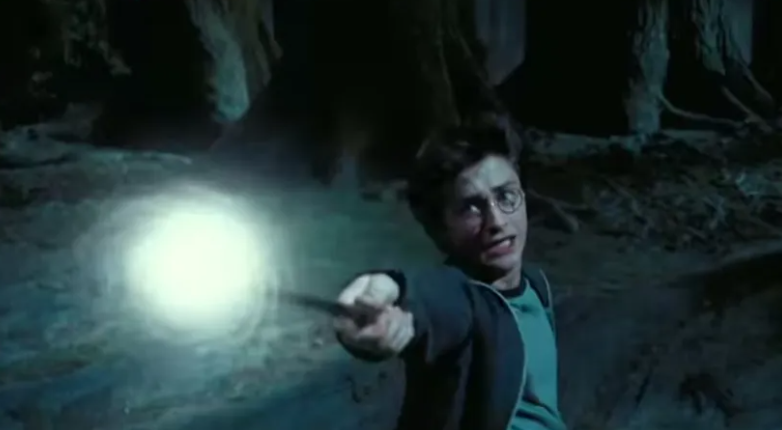
\includegraphics[width=6.17708in,height=\textheight,keepaspectratio]{clases/www/patronum.png}
\end{center}

\subsection{Los paquetes}\label{los-paquetes}

\begin{Shaded}
\begin{Highlighting}[]
\FunctionTok{library}\NormalTok{(tidyverse)}
\FunctionTok{library}\NormalTok{(janitor)}
\FunctionTok{library}\NormalTok{(tm)}
\FunctionTok{library}\NormalTok{(wordcloud)}
\end{Highlighting}
\end{Shaded}

\subsubsection{\texorpdfstring{\textbf{Sobre los
paquetes}}{Sobre los paquetes}}\label{sobre-los-paquetes}

\texttt{Tidyverse} es un~conjunto de paquetes de R. Se utiliza para
analizar datos y está compuesto por paquetes que comparten una filosofía
de diseño, gramática y estructura. Más información
\href{https://www.tidyverse.org/}{acá}

\begin{figure}[H]

{\centering \pandocbounded{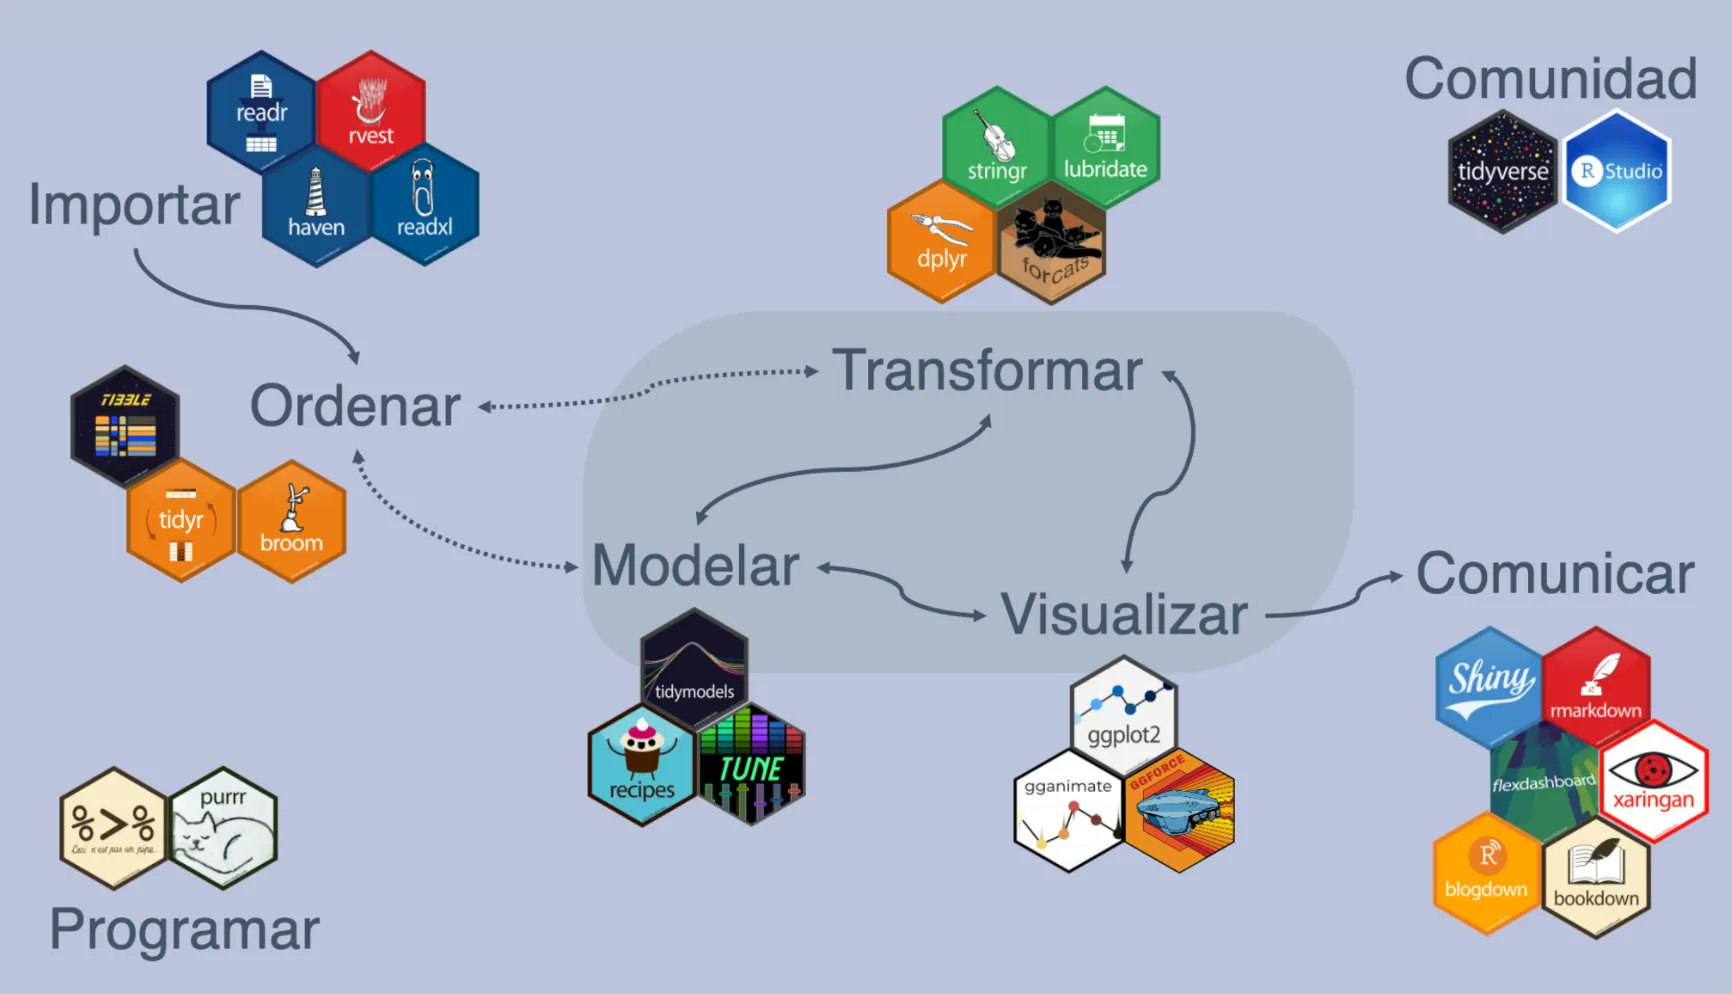
\includegraphics[keepaspectratio]{clases/www/tidyverse.jpg}}

}

\caption{Fuente:
https://x.com/RosanaFerrero/status/1521396654829617153/photo/1}

\end{figure}%

\texttt{esquisse} es un paquete que permite generar graficos con
\texttt{ggplot} a partir de una manera interactiva utilizando drag and
drop. Más información \href{https://dreamrs.github.io/esquisse/}{acá}

\texttt{janitor} contiene funciones para limpiar y examinar datos. Más
información
\href{https://www.rdocumentation.org/packages/janitor/versions/2.2.1}{acá}

\subsection{Cargamos el libro}\label{cargamos-el-libro}

\begin{Shaded}
\begin{Highlighting}[]
\CommentTok{\# Cargamos los datos}
\NormalTok{hp3 }\OtherTok{\textless{}{-}} \FunctionTok{readLines}\NormalTok{(}\StringTok{"data/hp3.txt"}\NormalTok{)}

\CommentTok{\# Lo convertimos en un solo vector}
\NormalTok{libro }\OtherTok{\textless{}{-}} \FunctionTok{paste}\NormalTok{(hp3, }\AttributeTok{collapse =} \StringTok{" "}\NormalTok{)}

\CommentTok{\# Vemos los primeros caracteres}
\FunctionTok{print}\NormalTok{(}\FunctionTok{substr}\NormalTok{(libro, }\DecValTok{1}\NormalTok{, }\DecValTok{500}\NormalTok{))  }
\end{Highlighting}
\end{Shaded}

\begin{verbatim}
[1] "J.K. Rowling Harry Potter y el prisionero de Azkaban   Por la cicatriz que lleva en la frente, sabemos que Harry Potter no es un niño como los demás, sino el héroe que venció a lord Voldemort, el mago más temible y maligno de todos los tiempos y culpable de la muerte de los padres de Harry. Desde entonces, Harry no tiene más remedio que vivir con sus pesados tíos y su insoportable primo Dudley, todos ellos muggles, o sea, personas no magas, que desprecian a su sobrino debido a sus poderes. Igual"
\end{verbatim}

\subsubsection{¿Cuantos caracteres tiene el
libro?}\label{cuantos-caracteres-tiene-el-libro}

\begin{Shaded}
\begin{Highlighting}[]
\CommentTok{\# ¿Cuantos caracteres tiene el libro? }
\FunctionTok{nchar}\NormalTok{(libro)}
\end{Highlighting}
\end{Shaded}

\begin{verbatim}
[1] 644726
\end{verbatim}

\subsubsection{¿Cuantas oraciones tiene el
libro?}\label{cuantas-oraciones-tiene-el-libro}

\begin{Shaded}
\begin{Highlighting}[]
\NormalTok{oraciones }\OtherTok{\textless{}{-}} \FunctionTok{unlist}\NormalTok{(}\FunctionTok{str\_split}\NormalTok{(libro, }\StringTok{"(?\textless{}=[.!?])}\SpecialCharTok{\textbackslash{}\textbackslash{}}\StringTok{s+"}\NormalTok{))}
\FunctionTok{length}\NormalTok{(oraciones)}
\end{Highlighting}
\end{Shaded}

\begin{verbatim}
[1] 10603
\end{verbatim}

\subsection{Frecuencia de palabras más
utilizadas}\label{frecuencia-de-palabras-muxe1s-utilizadas}

\subsubsection{Limpiamos el texto}\label{limpiamos-el-texto}

\texttt{gsub()} es una función en \textbf{R} que se usa para
\textbf{buscar y reemplazar texto} dentro de cadenas de caracteres.

La sintaxis es:

\begin{Shaded}
\begin{Highlighting}[]
\FunctionTok{gsub}\NormalTok{(}\StringTok{"patrón\_a\_buscar"}\NormalTok{, }\StringTok{"nuevo\_texto"}\NormalTok{, texto)}
\end{Highlighting}
\end{Shaded}

A través de esta función vamos a limpiar el texto del libro para mejorar
el conteo de las palabrbas

\begin{Shaded}
\begin{Highlighting}[]
\CommentTok{\# Convertimos a minusculas}
\NormalTok{libro\_limpio }\OtherTok{\textless{}{-}} \FunctionTok{tolower}\NormalTok{(libro)  }
\CommentTok{\# Eliminamos las puntuaciones}
\NormalTok{libro\_limpio }\OtherTok{\textless{}{-}} \FunctionTok{gsub}\NormalTok{(}\StringTok{"[[:punct:]]"}\NormalTok{, }\StringTok{""}\NormalTok{, libro\_limpio)  }
\CommentTok{\# Eliminamos los números}
\NormalTok{libro\_limpio }\OtherTok{\textless{}{-}} \FunctionTok{gsub}\NormalTok{(}\StringTok{"[[:digit:]]"}\NormalTok{, }\StringTok{""}\NormalTok{, libro\_limpio) }
\CommentTok{\# Eliminamos espacios múltiples}
\NormalTok{libro\_limpio }\OtherTok{\textless{}{-}} \FunctionTok{gsub}\NormalTok{(}\StringTok{"}\SpecialCharTok{\textbackslash{}\textbackslash{}}\StringTok{s+"}\NormalTok{, }\StringTok{" "}\NormalTok{, libro\_limpio) }
\NormalTok{libro\_limpio }\OtherTok{\textless{}{-}} \FunctionTok{gsub}\NormalTok{(}\StringTok{"[\^{}}\SpecialCharTok{\textbackslash{}x20}\StringTok{{-}}\SpecialCharTok{\textbackslash{}x7E}\StringTok{]"}\NormalTok{, }\StringTok{""}\NormalTok{, libro\_limpio)  }\CommentTok{\# Elimina caracteres no imprimibles}
\end{Highlighting}
\end{Shaded}

\subsubsection{Dividimos las palabras}\label{dividimos-las-palabras}

\begin{Shaded}
\begin{Highlighting}[]
\CommentTok{\# Divido las palabras:}

\NormalTok{palabras }\OtherTok{\textless{}{-}} \FunctionTok{unlist}\NormalTok{(}\FunctionTok{strsplit}\NormalTok{(libro\_limpio, }\StringTok{"}\SpecialCharTok{\textbackslash{}\textbackslash{}}\StringTok{s+"}\NormalTok{)) }
\end{Highlighting}
\end{Shaded}

\subsubsection{Eliminamos las stopwords}\label{eliminamos-las-stopwords}

Las stopwords (o palabras vacías) son palabras muy comunes en un idioma
que suelen tener poco valor en análisis de texto porque no aportan
significado relevante. Ejemplos en español incluyen:

🔹 Preposiciones: ``de'', ``a'', ``con'', ``por'', ``para'' 🔹
Artículos: ``el'', ``la'', ``los'', ``las'' 🔹 Conjunciones: ``y'',
``o'', ``pero'', ``aunque'' 🔹 Pronombres: ``yo'', ``tú'', ``él'',
``ella'', ``nosotros'' 🔹 Verbos auxiliares: ``ser'', ``estar'',
``haber''

\begin{Shaded}
\begin{Highlighting}[]
\NormalTok{stopwords\_es }\OtherTok{\textless{}{-}} \FunctionTok{stopwords}\NormalTok{(}\StringTok{"es"}\NormalTok{) }

\CommentTok{\# Vector sin los stopwords}
\NormalTok{palabras\_filtradas }\OtherTok{\textless{}{-}}\NormalTok{ palabras[}\SpecialCharTok{!}\NormalTok{palabras }\SpecialCharTok{\%in\%}\NormalTok{ stopwords\_es] }
\end{Highlighting}
\end{Shaded}

\subsubsection{Contamos}\label{contamos}

\begin{Shaded}
\begin{Highlighting}[]
\NormalTok{frecuencia }\OtherTok{\textless{}{-}} \FunctionTok{table}\NormalTok{(palabras\_filtradas)}
\CommentTok{\# Ordenamos por la frecuencia}
\NormalTok{frecuencia }\OtherTok{\textless{}{-}} \FunctionTok{sort}\NormalTok{(frecuencia, }\AttributeTok{decreasing =} \ConstantTok{TRUE}\NormalTok{) }

\CommentTok{\# Top 20 palabras}
\FunctionTok{head}\NormalTok{(frecuencia, }\DecValTok{20}\NormalTok{)}
\end{Highlighting}
\end{Shaded}

\begin{verbatim}
palabras_filtradas
    harry      dijo       ron  hermione      haba        si     lupin        ms 
     1935      1020       769       656       649       404       401       400 
       qu     black         l     hacia    hagrid     snape  profesor   pregunt 
      397       307       264       260       253       245       242       223 
      voz         s profesora    malfoy 
      222       206       203       185 
\end{verbatim}

\subsection{Graficamos}\label{graficamos}

\begin{enumerate}
\def\labelenumi{\arabic{enumi})}
\tightlist
\item
  Convertimos nuestras frecuencias en una tabla
\end{enumerate}

\begin{Shaded}
\begin{Highlighting}[]
\NormalTok{df\_frec }\OtherTok{\textless{}{-}} \FunctionTok{as.data.frame}\NormalTok{(frecuencia)}
\FunctionTok{colnames}\NormalTok{(df\_frec) }\OtherTok{\textless{}{-}} \FunctionTok{c}\NormalTok{(}\StringTok{"Palabra"}\NormalTok{, }\StringTok{"Frecuencia"}\NormalTok{)}


\FunctionTok{head}\NormalTok{(df\_frec)}
\end{Highlighting}
\end{Shaded}

\begin{verbatim}
   Palabra Frecuencia
1    harry       1935
2     dijo       1020
3      ron        769
4 hermione        656
5     haba        649
6       si        404
\end{verbatim}

Me quedo con las 20 palabras más mencionadas y grafico utilizando
\texttt{esquisser}

\begin{Shaded}
\begin{Highlighting}[]
\NormalTok{df\_grafico }\OtherTok{\textless{}{-}}\NormalTok{ df\_frec }\SpecialCharTok{|\textgreater{}} 
  \FunctionTok{head}\NormalTok{(}\DecValTok{20}\NormalTok{)}
\end{Highlighting}
\end{Shaded}

\begin{Shaded}
\begin{Highlighting}[]
\NormalTok{esquisse}\SpecialCharTok{::}\FunctionTok{esquisser}\NormalTok{(df\_grafico)}
\end{Highlighting}
\end{Shaded}

Lo diseñamos a gusto y luego guardamos el código

\begin{Shaded}
\begin{Highlighting}[]
\CommentTok{\# Grafico final}

\FunctionTok{ggplot}\NormalTok{(df\_grafico) }\SpecialCharTok{+}
  \FunctionTok{aes}\NormalTok{(}\AttributeTok{x =}\NormalTok{ Palabra, }\AttributeTok{y =}\NormalTok{ Frecuencia) }\SpecialCharTok{+}
  \FunctionTok{geom\_col}\NormalTok{(}\AttributeTok{fill =} \StringTok{"\#440154"}\NormalTok{) }\SpecialCharTok{+}
  \FunctionTok{labs}\NormalTok{(}
    \AttributeTok{x =} \StringTok{"Palabras"}\NormalTok{,}
    \AttributeTok{y =} \StringTok{"Cantidad"}\NormalTok{,}
    \AttributeTok{title =} \StringTok{"Palabras mas mencionadas en Harry Potter 3"}
\NormalTok{  ) }\SpecialCharTok{+}
\NormalTok{  ggthemes}\SpecialCharTok{::}\FunctionTok{theme\_fivethirtyeight}\NormalTok{() }\SpecialCharTok{+}
  \FunctionTok{theme}\NormalTok{(}
    \AttributeTok{legend.justification =} \StringTok{"top"}\NormalTok{,}
    \AttributeTok{plot.title =} \FunctionTok{element\_text}\NormalTok{(}\AttributeTok{size =} \DecValTok{14}\NormalTok{L,}
    \AttributeTok{face =} \StringTok{"bold"}\NormalTok{,}
    \AttributeTok{hjust =} \FloatTok{0.5}\NormalTok{)}
\NormalTok{  )}
\end{Highlighting}
\end{Shaded}

\pandocbounded{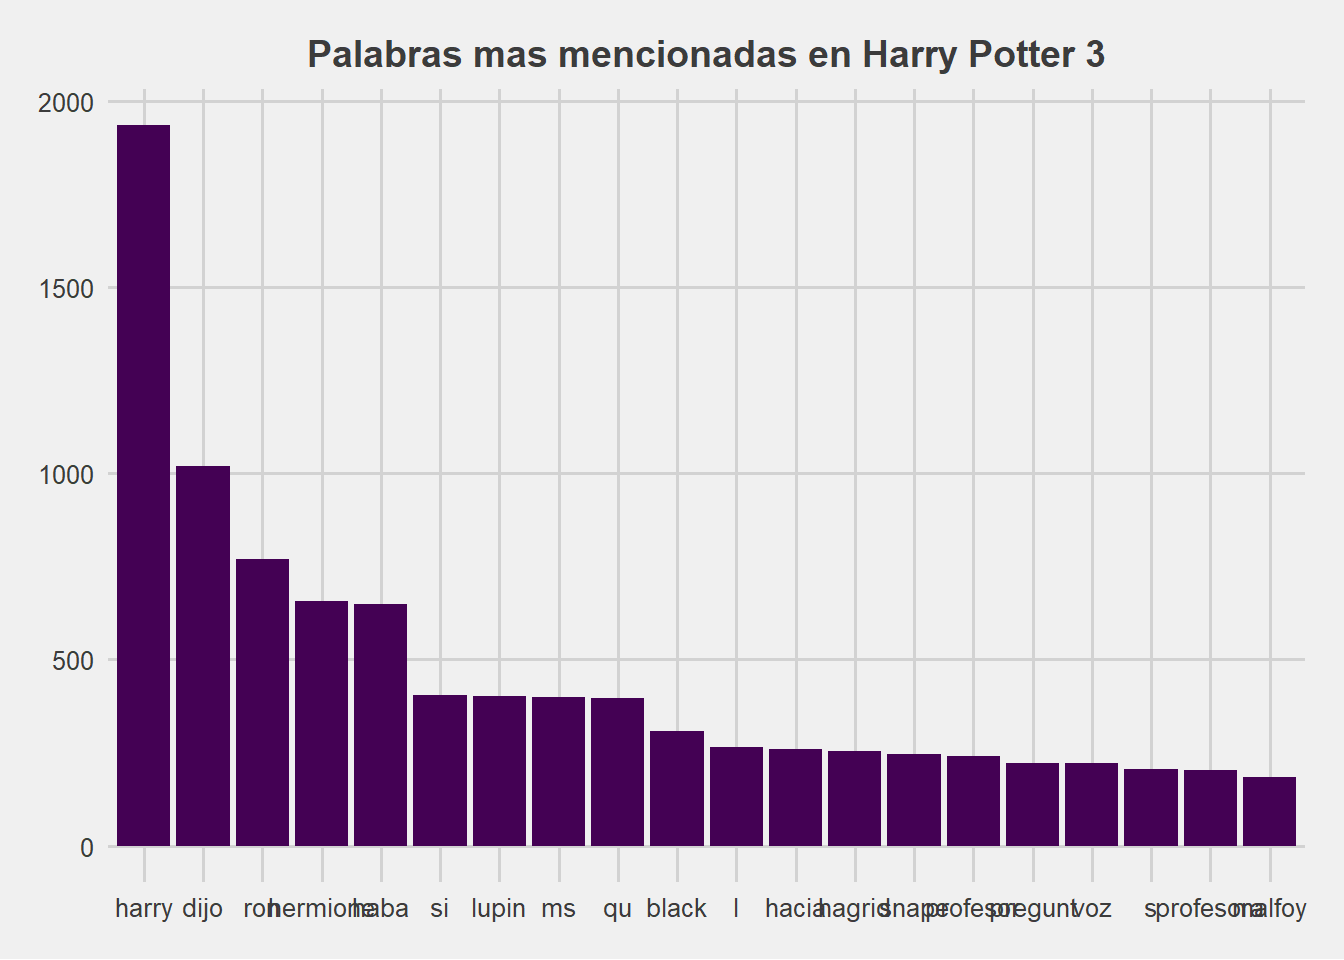
\includegraphics[keepaspectratio]{clases/clase1_T_files/figure-pdf/unnamed-chunk-11-1.pdf}}

\subsubsection{Nube de palabras}\label{nube-de-palabras}

También podemos realizar una nube de palabras:

\begin{Shaded}
\begin{Highlighting}[]
\FunctionTok{wordcloud}\NormalTok{(}\FunctionTok{names}\NormalTok{(frecuencia), frecuencia, }\AttributeTok{max.words =} \DecValTok{100}\NormalTok{, }\AttributeTok{colors =} \FunctionTok{brewer.pal}\NormalTok{(}\DecValTok{8}\NormalTok{, }\StringTok{"Dark2"}\NormalTok{))}
\end{Highlighting}
\end{Shaded}

\begin{verbatim}
Warning in wordcloud(names(frecuencia), frecuencia, max.words = 100, colors =
brewer.pal(8, : harry could not be fit on page. It will not be plotted.
\end{verbatim}

\pandocbounded{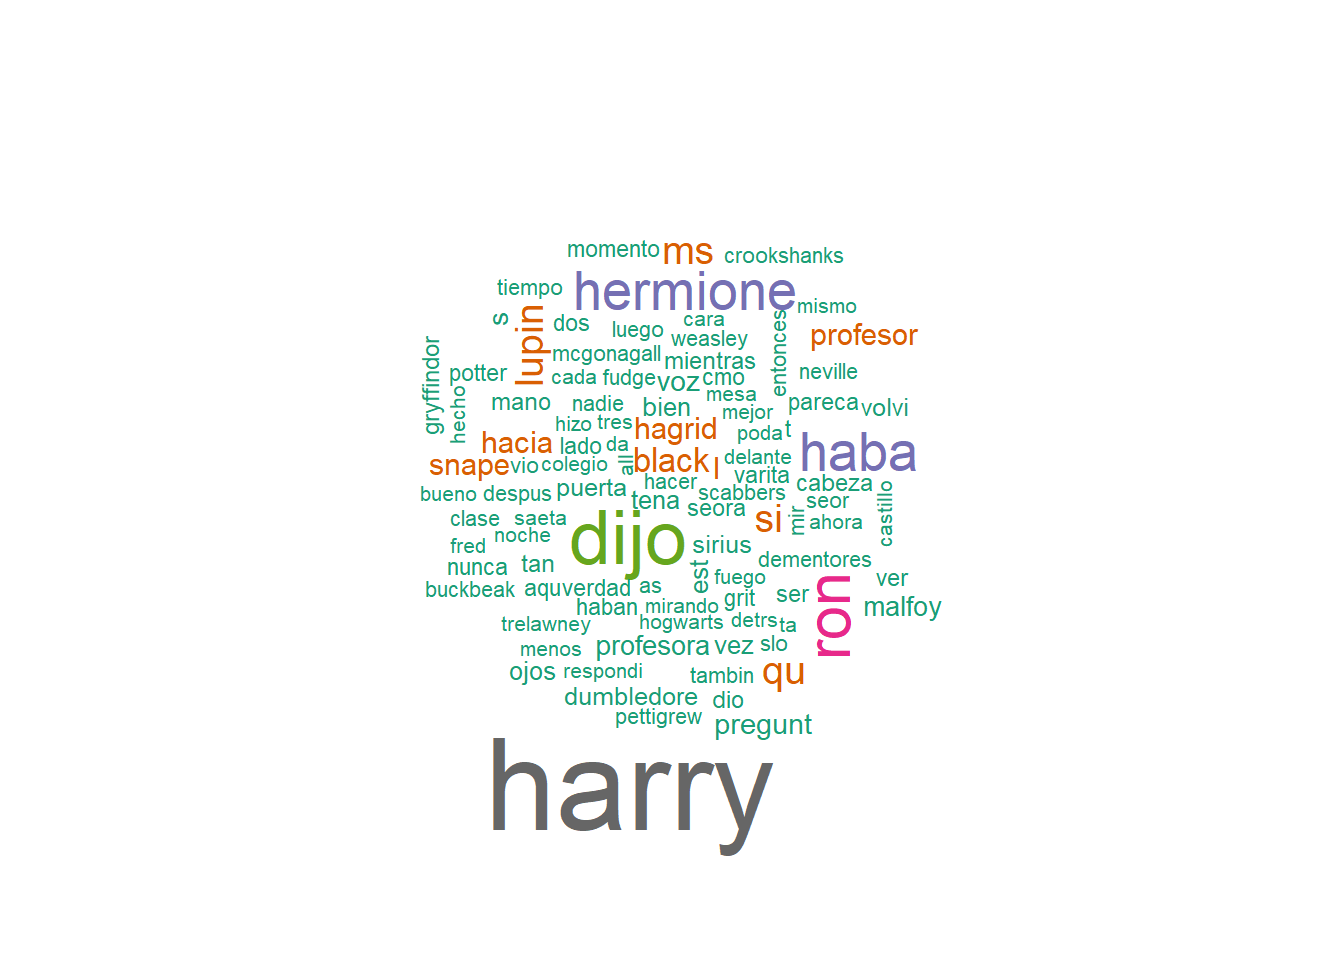
\includegraphics[keepaspectratio]{clases/clase1_T_files/figure-pdf/unnamed-chunk-12-1.pdf}}

\part{\textbf{Clase 2. Expresiones regulares}}

\chapter{C2. Presentación}\label{c2.-presentaciuxf3n}

\section{\texorpdfstring{\textbf{Objetivo de la
clase}}{Objetivo de la clase}}\label{objetivo-de-la-clase-1}

En esta clase aprenderemos a utilizar expresiones regulares para la
extracción y manipulación de texto libre

\section{\texorpdfstring{\textbf{Presentación}}{Presentación}}\label{presentaciuxf3n-1}

\chapter{C2. Taller Práctico}\label{c2.-taller-pruxe1ctico}

El \textbf{Servicio de Información Normativa} es un conjunto de datos
publicado por el Gobierno de la Ciudad Autónoma de Buenos Aires. Este
dataset recopila las normativas sancionadas en el ámbito de la ciudad,
publicadas tanto en el Boletín Municipal como en el Boletín Oficial
desde el 6 de agosto de 1996.

\href{https://data.buenosaires.gob.ar/dataset/servicio-informacion-normativa?utm_source=chatgpt.com}{data.buenosaires.gob.ar}

\begin{Shaded}
\begin{Highlighting}[]
\FunctionTok{library}\NormalTok{(tidyverse)}
\end{Highlighting}
\end{Shaded}

\begin{verbatim}
Warning: package 'tidyverse' was built under R version 4.3.3
\end{verbatim}

\begin{verbatim}
Warning: package 'ggplot2' was built under R version 4.3.3
\end{verbatim}

\begin{verbatim}
Warning: package 'readr' was built under R version 4.3.3
\end{verbatim}

\begin{verbatim}
Warning: package 'dplyr' was built under R version 4.3.2
\end{verbatim}

\begin{verbatim}
-- Attaching core tidyverse packages ------------------------ tidyverse 2.0.0 --
v dplyr     1.1.4     v readr     2.1.5
v forcats   1.0.0     v stringr   1.5.0
v ggplot2   3.5.1     v tibble    3.2.1
v lubridate 1.9.3     v tidyr     1.3.0
v purrr     1.0.2     
-- Conflicts ------------------------------------------ tidyverse_conflicts() --
x dplyr::filter() masks stats::filter()
x dplyr::lag()    masks stats::lag()
i Use the conflicted package (<http://conflicted.r-lib.org/>) to force all conflicts to become errors
\end{verbatim}

\begin{Shaded}
\begin{Highlighting}[]
\FunctionTok{library}\NormalTok{(janitor)}
\end{Highlighting}
\end{Shaded}

\begin{verbatim}
Warning: package 'janitor' was built under R version 4.3.3
\end{verbatim}

\begin{verbatim}

Attaching package: 'janitor'

The following objects are masked from 'package:stats':

    chisq.test, fisher.test
\end{verbatim}

\begin{Shaded}
\begin{Highlighting}[]
\NormalTok{df\_normativa }\OtherTok{\textless{}{-}} \FunctionTok{read\_csv}\NormalTok{(}\StringTok{"https://cdn.buenosaires.gob.ar/datosabiertos/datasets/secretaria{-}legal{-}y{-}tecnica/servicio{-}informacion{-}normativa/normativa.csv"}\NormalTok{) }\SpecialCharTok{|\textgreater{}} 
  \FunctionTok{clean\_names}\NormalTok{()}
\end{Highlighting}
\end{Shaded}

\begin{verbatim}
Warning: One or more parsing issues, call `problems()` on your data frame for details,
e.g.:
  dat <- vroom(...)
  problems(dat)
\end{verbatim}

\begin{verbatim}
Rows: 748671 Columns: 11
-- Column specification --------------------------------------------------------
Delimiter: ","
chr (7): norma_tipo, norma_organismo_emisor, norma_fecha_sancion, norma_fech...
dbl (4): norma_id, norma_numero, norma_anio_sancion, norma_anio_publicacion

i Use `spec()` to retrieve the full column specification for this data.
i Specify the column types or set `show_col_types = FALSE` to quiet this message.
\end{verbatim}

Antes de empezar a trabajar con expresiones regulares vamos a analizar
un poco la base

\begin{Shaded}
\begin{Highlighting}[]
\FunctionTok{glimpse}\NormalTok{(df\_normativa)}
\end{Highlighting}
\end{Shaded}

\begin{verbatim}
Rows: 748,671
Columns: 11
$ norma_id                <dbl> 78404, 78405, 78406, 78407, 78408, 78409, 7841~
$ norma_tipo              <chr> "DECRETO SINTETIZADO", "DECRETO SINTETIZADO", ~
$ norma_numero            <dbl> 1570, 1574, 1576, 1577, 1579, 1591, 1596, 1597~
$ norma_anio_sancion      <dbl> 2005, 2005, 2005, 2005, 2005, 2005, 2005, 2005~
$ norma_anio_publicacion  <dbl> 2005, 2005, 2005, 2005, 2005, 2005, 2005, 2005~
$ norma_organismo_emisor  <chr> "GOBIERNO DE LA CIUDAD AUTONOMA DE BUENOS AIRE~
$ norma_fecha_sancion     <chr> "14/10/2005", "14/10/2005", "14/10/2005", "14/~
$ norma_fecha_publicacion <chr> "31/10/2005", "31/10/2005", "31/10/2005", "31/~
$ norma_alcance           <chr> "PARTICULAR", "PARTICULAR", "PARTICULAR", "PAR~
$ norma_gestion           <chr> "Aníbal Ibarra", "Aníbal Ibarra", "Aníbal Ibar~
$ norma_sintesis          <chr> "SECRETARÍA JEFE DE GABINETE - DESIGNA A GENOV~
\end{verbatim}

\begin{Shaded}
\begin{Highlighting}[]
\FunctionTok{summary}\NormalTok{(df\_normativa)}
\end{Highlighting}
\end{Shaded}

\begin{verbatim}
    norma_id       norma_tipo         norma_numero       norma_anio_sancion
 Min.   :     1   Length:748671      Min.   :        0   Min.   :1858      
 1st Qu.:190912   Class :character   1st Qu.:      129   1st Qu.:2011      
 Median :380912   Mode  :character   Median :      427   Median :2017      
 Mean   :380335                      Mean   :   415450   Mean   :2015      
 3rd Qu.:570305                      3rd Qu.:     1511   3rd Qu.:2021      
 Max.   :757614                      Max.   :141182503   Max.   :2027      
                                     NA's   :2282        NA's   :412       
 norma_anio_publicacion norma_organismo_emisor norma_fecha_sancion
 Min.   :1882           Length:748671          Length:748671      
 1st Qu.:2012           Class :character       Class :character   
 Median :2017           Mode  :character       Mode  :character   
 Mean   :2016                                                     
 3rd Qu.:2021                                                     
 Max.   :2202                                                     
 NA's   :8834                                                     
 norma_fecha_publicacion norma_alcance      norma_gestion     
 Length:748671           Length:748671      Length:748671     
 Class :character        Class :character   Class :character  
 Mode  :character        Mode  :character   Mode  :character  
                                                              
                                                              
                                                              
                                                              
 norma_sintesis    
 Length:748671     
 Class :character  
 Mode  :character  
                   
                   
                   
                   
\end{verbatim}

¿Qué tipos de normativa existen?

\begin{Shaded}
\begin{Highlighting}[]
\NormalTok{df\_normativa }\SpecialCharTok{|\textgreater{}} 
  \FunctionTok{count}\NormalTok{(norma\_tipo, }\AttributeTok{sort =} \ConstantTok{TRUE}\NormalTok{) }\SpecialCharTok{|\textgreater{}} 
  \FunctionTok{view}\NormalTok{()}

\NormalTok{df\_normativa }\SpecialCharTok{|\textgreater{}} 
  \FunctionTok{count}\NormalTok{(norma\_anio\_sancion)}
\end{Highlighting}
\end{Shaded}

\begin{verbatim}
# A tibble: 148 x 2
   norma_anio_sancion     n
                <dbl> <int>
 1               1858     1
 2               1867     1
 3               1869     1
 4               1870     1
 5               1872     1
 6               1876     1
 7               1880     1
 8               1881     1
 9               1882     1
10               1883     1
# i 138 more rows
\end{verbatim}

\subsection{Ejercicio 1: Filtrar normativas sobre Locaciones de Obras y
Servicios
(LOYS)}\label{ejercicio-1-filtrar-normativas-sobre-locaciones-de-obras-y-servicios-loys}

El objetivo es Filtrar todas las normativas referidas a contrataciones
de locaciones de obras y servicios (LOYS).

\begin{Shaded}
\begin{Highlighting}[]
\NormalTok{patron\_loys }\OtherTok{\textless{}{-}} \FunctionTok{regex}\NormalTok{(}\StringTok{"}\SpecialCharTok{\textbackslash{}\textbackslash{}}\StringTok{bloys}\SpecialCharTok{\textbackslash{}\textbackslash{}}\StringTok{b|locaci.n ?de obras y servicios"}\NormalTok{, T)}
\NormalTok{patron\_baja\_contrato }\OtherTok{\textless{}{-}} \FunctionTok{regex}\NormalTok{(}\StringTok{"deja sin efecto|}\SpecialCharTok{\textbackslash{}\textbackslash{}}\StringTok{bbaja"}\NormalTok{,T)}
\NormalTok{aumento }\OtherTok{\textless{}{-}} \FunctionTok{regex}\NormalTok{(}\StringTok{"(aumenta|eleva|sube).\{0,20\} monto"}\NormalTok{,T)}

\CommentTok{\# Me quedo con todas normativas vinculadas a loys}
\NormalTok{loys }\OtherTok{\textless{}{-}}\NormalTok{ df\_normativa  }\SpecialCharTok{|\textgreater{}} 
  \FunctionTok{filter}\NormalTok{(}\FunctionTok{str\_detect}\NormalTok{(norma\_sintesis, patron\_loys))}

\NormalTok{loys }\SpecialCharTok{|\textgreater{}} 
  \FunctionTok{count}\NormalTok{(norma\_anio\_sancion)}
\end{Highlighting}
\end{Shaded}

\begin{verbatim}
# A tibble: 14 x 2
   norma_anio_sancion     n
                <dbl> <int>
 1               2006     1
 2               2011     4
 3               2012     3
 4               2013     6
 5               2014     6
 6               2015     6
 7               2016     6
 8               2018     8
 9               2019     8
10               2020    11
11               2021     9
12               2022     8
13               2023    18
14               2024    11
\end{verbatim}

\subsubsection{1.1 Clasificar las normativas
LOYS}\label{clasificar-las-normativas-loys}

Ahora vamos a caracterizar las normativas LOYS según su tipo:

\begin{itemize}
\item
  Alta: Contrataciones nuevas
\item
  Baja: Rescisión de contrato
\item
  Adenda: Aumento del monto del contrato
\end{itemize}

\begin{Shaded}
\begin{Highlighting}[]
\NormalTok{loys }\OtherTok{\textless{}{-}}\NormalTok{ df\_normativa  }\SpecialCharTok{|\textgreater{}} 
  \FunctionTok{filter}\NormalTok{(}\FunctionTok{str\_detect}\NormalTok{(norma\_sintesis, patron\_loys)) }\SpecialCharTok{|\textgreater{}} 
  \FunctionTok{mutate}\NormalTok{(}\AttributeTok{tipo\_normativa\_loys =} \FunctionTok{case\_when}\NormalTok{(}\FunctionTok{str\_detect}\NormalTok{(norma\_sintesis, patron\_baja\_contrato) }\SpecialCharTok{\textasciitilde{}} \StringTok{"Baja"}\NormalTok{,}
                                         \FunctionTok{str\_detect}\NormalTok{(norma\_sintesis, aumento) }\SpecialCharTok{\textasciitilde{}}\StringTok{"Adenda"}\NormalTok{,}
\NormalTok{                                                   T }\SpecialCharTok{\textasciitilde{}} \StringTok{"Alta"}
\NormalTok{                                         ))}

\CommentTok{\# Grafico}
\NormalTok{loys }\SpecialCharTok{|\textgreater{}} 
  \FunctionTok{count}\NormalTok{(tipo\_normativa\_loys, }\AttributeTok{sort =} \ConstantTok{TRUE}\NormalTok{) }\SpecialCharTok{|\textgreater{}} 
  \FunctionTok{ggplot}\NormalTok{(}\FunctionTok{aes}\NormalTok{(}\AttributeTok{x =} \FunctionTok{reorder}\NormalTok{(tipo\_normativa\_loys, n), }\AttributeTok{y =}\NormalTok{ n)) }\SpecialCharTok{+}
  \FunctionTok{geom\_col}\NormalTok{(}\AttributeTok{fill =} \StringTok{"steelblue"}\NormalTok{) }\SpecialCharTok{+}
  \FunctionTok{coord\_flip}\NormalTok{() }\SpecialCharTok{+}
  \FunctionTok{labs}\NormalTok{(}
    \AttributeTok{title =} \StringTok{"Distribución de tipos de normativas en LOYS"}\NormalTok{,}
    \AttributeTok{x =} \StringTok{"Tipo de normativa"}\NormalTok{,}
    \AttributeTok{y =} \StringTok{"Cantidad"}
\NormalTok{  ) }\SpecialCharTok{+}
  \FunctionTok{theme\_minimal}\NormalTok{()}
\end{Highlighting}
\end{Shaded}

\pandocbounded{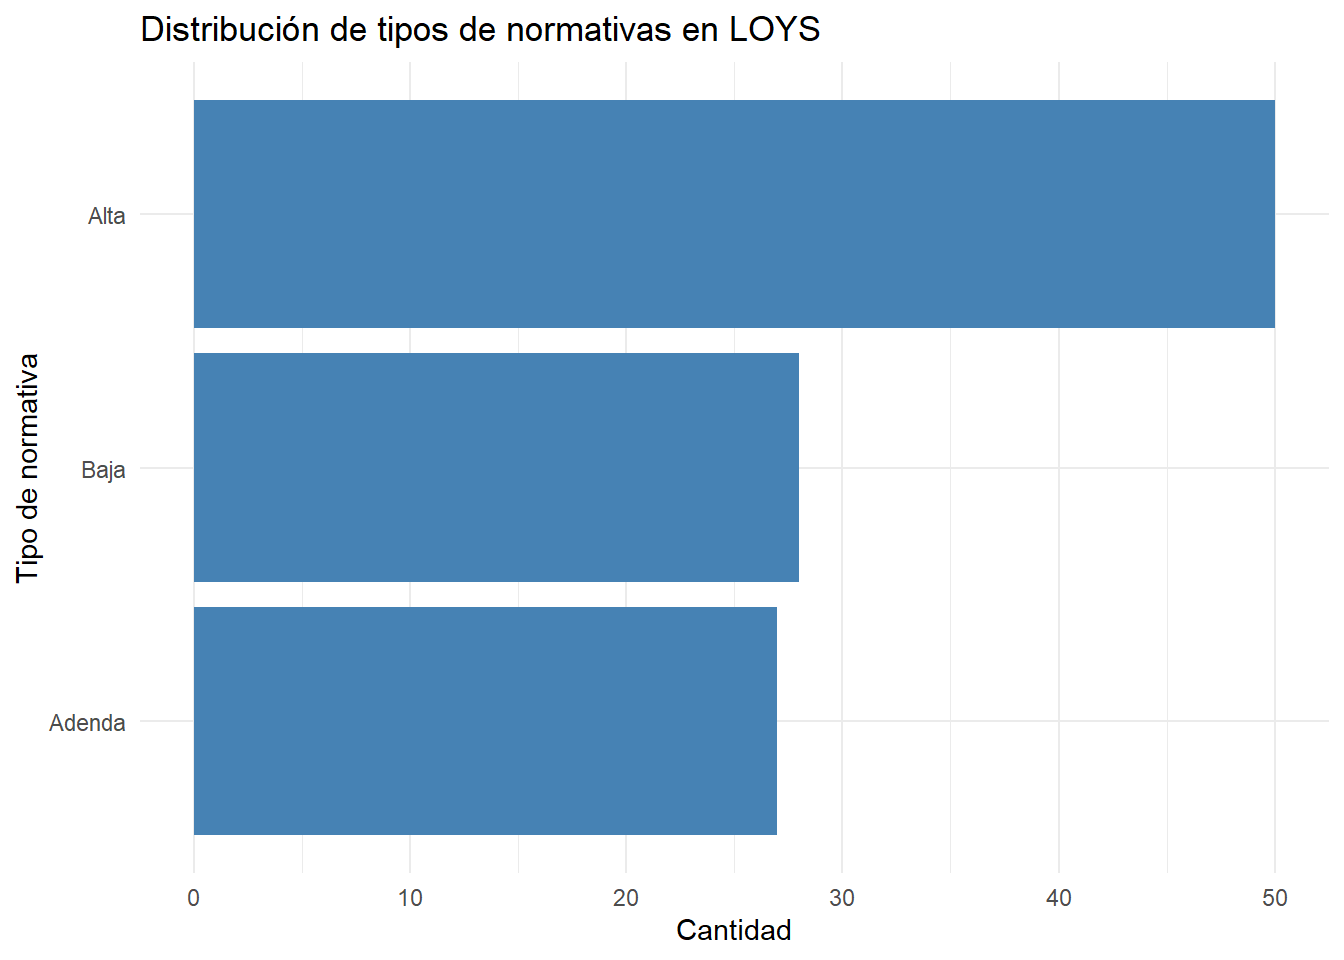
\includegraphics[keepaspectratio]{clases/clase2_T_files/figure-pdf/unnamed-chunk-5-1.pdf}}

\subsection{Ejercicio 2: Filtrar designaciones y
renuncias}\label{ejercicio-2-filtrar-designaciones-y-renuncias}

\subsubsection{Objetivo}\label{objetivo}

Filtrar todas las normativas que mencionen \textbf{designaciones} y
\textbf{renuncias} de personal.

\subsubsection{\texorpdfstring{\textbf{Paso 1: Filtrar la base de datos
por designaciones y
renuncia}}{Paso 1: Filtrar la base de datos por designaciones y renuncia}}\label{paso-1-filtrar-la-base-de-datos-por-designaciones-y-renuncia}

Completar los patrones regex

\begin{Shaded}
\begin{Highlighting}[]
\NormalTok{patron\_renuncia }\OtherTok{\textless{}{-}} \FunctionTok{regex}\NormalTok{(}\StringTok{""}\NormalTok{, T)  }\CommentTok{\# 📝 Completar }
\NormalTok{patron\_designacion }\OtherTok{\textless{}{-}} \FunctionTok{regex}\NormalTok{(}\StringTok{""}\NormalTok{ , T)  }\CommentTok{\# 📝 Completar }

\NormalTok{df\_renuncias\_y\_designaciones }\OtherTok{\textless{}{-}}\NormalTok{ df\_normativa }\SpecialCharTok{|\textgreater{}} 
  \CommentTok{\# Filtro}
  \FunctionTok{filter}\NormalTok{(}\FunctionTok{str\_detect}\NormalTok{(norma\_sintesis, patron\_renuncia) }\SpecialCharTok{|} \FunctionTok{str\_detect}\NormalTok{(norma\_sintesis, patron\_renuncia))}
\end{Highlighting}
\end{Shaded}

\begin{verbatim}
Warning: There were 2 warnings in `filter()`.
The first warning was:
i In argument: `|...`.
Caused by warning in `stri_detect_regex()`:
! empty search patterns are not supported
i Run `dplyr::last_dplyr_warnings()` to see the 1 remaining warning.
\end{verbatim}

\subsubsection{\texorpdfstring{\textbf{Paso 2: Clasificar en renuncias o
designaciones}}{Paso 2: Clasificar en renuncias o designaciones}}\label{paso-2-clasificar-en-renuncias-o-designaciones}

\begin{Shaded}
\begin{Highlighting}[]
 \CommentTok{\# 📝 Completar }
 \CommentTok{\# PISTA: Podes usar case\_when() o ifelse()}
\end{Highlighting}
\end{Shaded}

\subsubsection{\texorpdfstring{\textbf{Paso 3: Extraer el
cargo}}{Paso 3: Extraer el cargo}}\label{paso-3-extraer-el-cargo}

Usamos \texttt{str\_extract()} para identificar el cargo mencionado en
la normativa.

Ejemplo: se podrían extraer las gerencias, subgerencias y secretarías

\begin{Shaded}
\begin{Highlighting}[]
\CommentTok{\# 📝 Completar}
\end{Highlighting}
\end{Shaded}

\subsubsection{\texorpdfstring{\textbf{Paso 4: Analizar los
resultados}}{Paso 4: Analizar los resultados}}\label{paso-4-analizar-los-resultados}

¿Hay algún dato interesante? ¿Hubo diferencia por año?

\begin{Shaded}
\begin{Highlighting}[]
\CommentTok{\# 📝 Completar}
\end{Highlighting}
\end{Shaded}

\subsection{}\label{section}

\chapter{C2: Actividad entregable}\label{c2-actividad-entregable}

\subsection{Ejercicio: Pensando en el trabajo
final}\label{ejercicio-pensando-en-el-trabajo-final}

📌 Buscar un tema de interés y un dataset relevante para plantear la
investigación final.

\begin{itemize}
\item
  Es requisito que sea un tema donde tengas que aplicar minería de
  texto.
\item
  Buscar un dataset o corpus relacionado con ese tema. Puede ser una
  página web, una API o incluso un video de youtube!
\end{itemize}

Algunos repositorios:

\begin{itemize}
\tightlist
\item
  \href{https://data.buenosaires.gob.ar/}{Datos Abiertos de Buenos
  Aires}
\end{itemize}

\begin{itemize}
\tightlist
\item
  \href{https://datos.gob.ar/}{Datos Abiertos de Argentina}
\end{itemize}

\begin{itemize}
\item
  \url{https://www.kaggle.com/}
\item
  \url{https://github.com/cienciadedatos/datos-de-miercoles}
\item
  \href{https://huggingface.co/collections/somosnlp/corpus-instructions-in-spanish-and-related-languages-6697e4ce5ef2828a1ff26d5d}{Corpus
  de NLP en español}
\end{itemize}

\section{Formato de entrega}\label{formato-de-entrega}

Documento que explique brevemente la temática seleccionada junto a una
descripción del dataset o corpus elegido.

\chapter{C2. Hoja de ruta de Expresiones Regulares en
R}\label{c2.-hoja-de-ruta-de-expresiones-regulares-en-r}

\chapter{Anclas}\label{anclas}

\begin{longtable}[]{@{}
  >{\raggedright\arraybackslash}p{(\linewidth - 2\tabcolsep) * \real{0.1549}}
  >{\raggedright\arraybackslash}p{(\linewidth - 2\tabcolsep) * \real{0.8451}}@{}}
\toprule\noalign{}
\begin{minipage}[b]{\linewidth}\raggedright
Expresión
\end{minipage} & \begin{minipage}[b]{\linewidth}\raggedright
Descripción
\end{minipage} \\
\midrule\noalign{}
\endhead
\bottomrule\noalign{}
\endlastfoot
\texttt{\^{}} & Inicio de la cadena o inicio de línea en patrón
multilínea \\
\texttt{\textbackslash{}\textbackslash{}A} & Inicio de la cadena \\
\texttt{\$} & Fin de la cadena o fin de línea en patrón multilínea \\
\texttt{\textbackslash{}\textbackslash{}Z} & Fin de la cadena \\
\texttt{\textbackslash{}\textbackslash{}b} & Límite de palabra \\
\texttt{\textbackslash{}\textbackslash{}B} & No límite de palabra \\
\texttt{\textbackslash{}\textbackslash{}\textless{}} & Inicio de
palabra \\
\texttt{\textbackslash{}\textbackslash{}\textgreater{}} & Fin de
palabra \\
\end{longtable}

\chapter{Clases de Caracteres}\label{clases-de-caracteres}

\begin{longtable}[]{@{}ll@{}}
\toprule\noalign{}
Expresión & Descripción \\
\midrule\noalign{}
\endhead
\bottomrule\noalign{}
\endlastfoot
\texttt{\textbackslash{}\textbackslash{}c} & Carácter de control \\
\texttt{\textbackslash{}\textbackslash{}s} & Espacio en blanco \\
\texttt{\textbackslash{}\textbackslash{}S} & No espacio en blanco \\
\texttt{\textbackslash{}\textbackslash{}d} & Dígito \\
\texttt{\textbackslash{}\textbackslash{}D} & No dígito \\
\texttt{\textbackslash{}\textbackslash{}w} & Carácter de palabra \\
\texttt{\textbackslash{}\textbackslash{}W} & No carácter de palabra \\
\texttt{\textbackslash{}\textbackslash{}x} & Dígito hexadecimal \\
\texttt{\textbackslash{}\textbackslash{}O} & Dígito octal \\
\end{longtable}

\chapter{POSIX}\label{posix}

\begin{longtable}[]{@{}ll@{}}
\toprule\noalign{}
Expresión & Descripción \\
\midrule\noalign{}
\endhead
\bottomrule\noalign{}
\endlastfoot
\texttt{{[}:upper:{]}} & Letras mayúsculas \\
\texttt{{[}:lower:{]}} & Letras minúsculas \\
\texttt{{[}:alpha:{]}} & Todas las letras \\
\texttt{{[}:alnum:{]}} & Letras y números \\
\texttt{{[}:digit:{]}} & Dígitos \\
\texttt{{[}:xdigit:{]}} & Dígitos hexadecimales \\
\texttt{{[}:punct:{]}} & Signos de puntuación \\
\texttt{{[}:blank:{]}} & Espacio y tabulación \\
\texttt{{[}:space:{]}} & Caracteres en blanco \\
\texttt{{[}:cntrl:{]}} & Caracteres de control \\
\texttt{{[}:graph:{]}} & Caracteres imprimibles \\
\texttt{{[}:print:{]}} & Caracteres imprimibles y espacios \\
\texttt{{[}:word:{]}} & Letras, números y guion bajo \\
\end{longtable}

\chapter{Aserciones}\label{aserciones}

\begin{longtable}[]{@{}ll@{}}
\toprule\noalign{}
Expresión & Descripción \\
\midrule\noalign{}
\endhead
\bottomrule\noalign{}
\endlastfoot
\texttt{?=} & Aserción de anticipación \\
\texttt{?!} & Aserción de anticipación negativa \\
\texttt{?\textless{}=} & Aserción de retroceso \\
\texttt{?!=} o \texttt{?!\textless{}} & Aserción de retroceso
negativa \\
\texttt{?\textgreater{}} & Subexpresión de una sola vez \\
\texttt{?()} & Condición (si-entonces) \\
\texttt{?()\textbar{}} & Condición (si-entonces-sino) \\
\texttt{?\#} & Comentario \\
\end{longtable}

\chapter{Cuantificadores}\label{cuantificadores}

\begin{longtable}[]{@{}ll@{}}
\toprule\noalign{}
Expresión & Descripción \\
\midrule\noalign{}
\endhead
\bottomrule\noalign{}
\endlastfoot
\texttt{*} & 0 o más veces \\
\texttt{\{3\}} & Exactamente 3 veces \\
\texttt{+} & 1 o más veces \\
\texttt{\{3,\}} & 3 o más veces \\
\texttt{?} & 0 o 1 vez \\
\texttt{\{3,5\}} & Entre 3 y 5 veces \\
\end{longtable}

Para hacer un cuantificador no codicioso, agregar \texttt{?} después.

\chapter{Grupos y Rangos}\label{grupos-y-rangos}

\begin{longtable}[]{@{}ll@{}}
\toprule\noalign{}
Expresión & Descripción \\
\midrule\noalign{}
\endhead
\bottomrule\noalign{}
\endlastfoot
\texttt{.} & Cualquier carácter excepto nueva línea \\
\texttt{(a\textbar{}b)} & \texttt{a} o \texttt{b} \\
\texttt{(...)} & Grupo \\
\texttt{(?:...)} & Grupo no capturante \\
\texttt{{[}abc{]}} & \texttt{a}, \texttt{b} o \texttt{c} \\
\texttt{{[}\^{}abc{]}} & No \texttt{a}, \texttt{b} o \texttt{c} \\
\texttt{{[}a-q{]}} & Letra minúscula de \texttt{a} a \texttt{q} \\
\texttt{{[}A-Q{]}} & Letra mayúscula de \texttt{A} a \texttt{Q} \\
\texttt{{[}0-7{]}} & Dígito de \texttt{0} a \texttt{7} \\
\end{longtable}

Los rangos son inclusivos. \textbar{}

\chapter{Reemplazo de Cadenas}\label{reemplazo-de-cadenas}

\begin{longtable}[]{@{}ll@{}}
\toprule\noalign{}
Expresión & Descripción \\
\midrule\noalign{}
\endhead
\bottomrule\noalign{}
\endlastfoot
\texttt{\$n} & \texttt{n}-ésimo grupo no pasivo \\
\texttt{\$2} & ``xyz'' en \texttt{/\^{}(abc(xyz))\$/} \\
\texttt{\$1} & ``xyz'' en \texttt{/\^{}(?:abc)(xyz)\$/} \\
`\texttt{\$} & Antes de la cadena coincidente \\
\texttt{\$\textquotesingle{}} & Después de la cadena coincidente \\
\texttt{\$+} & Última coincidencia \\
\texttt{\$\&} & Cadena coincidente completa \\
\end{longtable}

\part{\textbf{Clase 3. Fuentes de datos textuales: APIS, Subtítulos y
PDFs}}

\chapter{C3. Antes de la clase}\label{c3.-antes-de-la-clase}

Antes de la clase no olvides tener los siguientes pasos hechos:

\chapter{Instalar las librerías}\label{instalar-las-libreruxedas}

Instalá los siguientes paquetes copiando y pegando el siguiente código
en la consola de RStudio:

\begin{Shaded}
\begin{Highlighting}[]

\NormalTok{paquetes\_lista }\OtherTok{\textless{}{-}} \FunctionTok{c}\NormalTok{(}
  \StringTok{"curl"}\NormalTok{, }\StringTok{"remotes"}\NormalTok{, }\StringTok{"spotifyr"}\NormalTok{, }\StringTok{"rjson"}\NormalTok{, }\StringTok{"gt"}\NormalTok{, }\StringTok{"reticulate"}\NormalTok{, }\StringTok{"pdftools"}
\NormalTok{)}

\FunctionTok{install.packages}\NormalTok{(paquetes\_lista)}
\end{Highlighting}
\end{Shaded}

Para descargar los subtítulos de youtube necesitarás

\begin{Shaded}
\begin{Highlighting}[]
\NormalTok{remotes}\SpecialCharTok{::}\FunctionTok{install\_github}\NormalTok{(}\StringTok{"jooyoungseo/youtubecaption"}\NormalTok{)}
\end{Highlighting}
\end{Shaded}

Si NO tenes el entorno de anaconda instalado tenes que correr el
siguiente comando en R

\begin{Shaded}
\begin{Highlighting}[]
\NormalTok{reticulate}\SpecialCharTok{::}\FunctionTok{install\_miniconda}\NormalTok{()}
\end{Highlighting}
\end{Shaded}

\chapter{Generar los usuario de la API de
Spotify}\label{generar-los-usuario-de-la-api-de-spotify}

Es necesario tener generado el usuario con las \textbf{credenciales de
la API de Spotify}

\subsection{1) Iniciar sesión en
https://developer.spotify.com/}\label{iniciar-sesiuxf3n-en-httpsdeveloper.spotify.com}

\section[ 2) Ingresa a la solapa de
Dashboards]{\texorpdfstring{\protect\pandocbounded{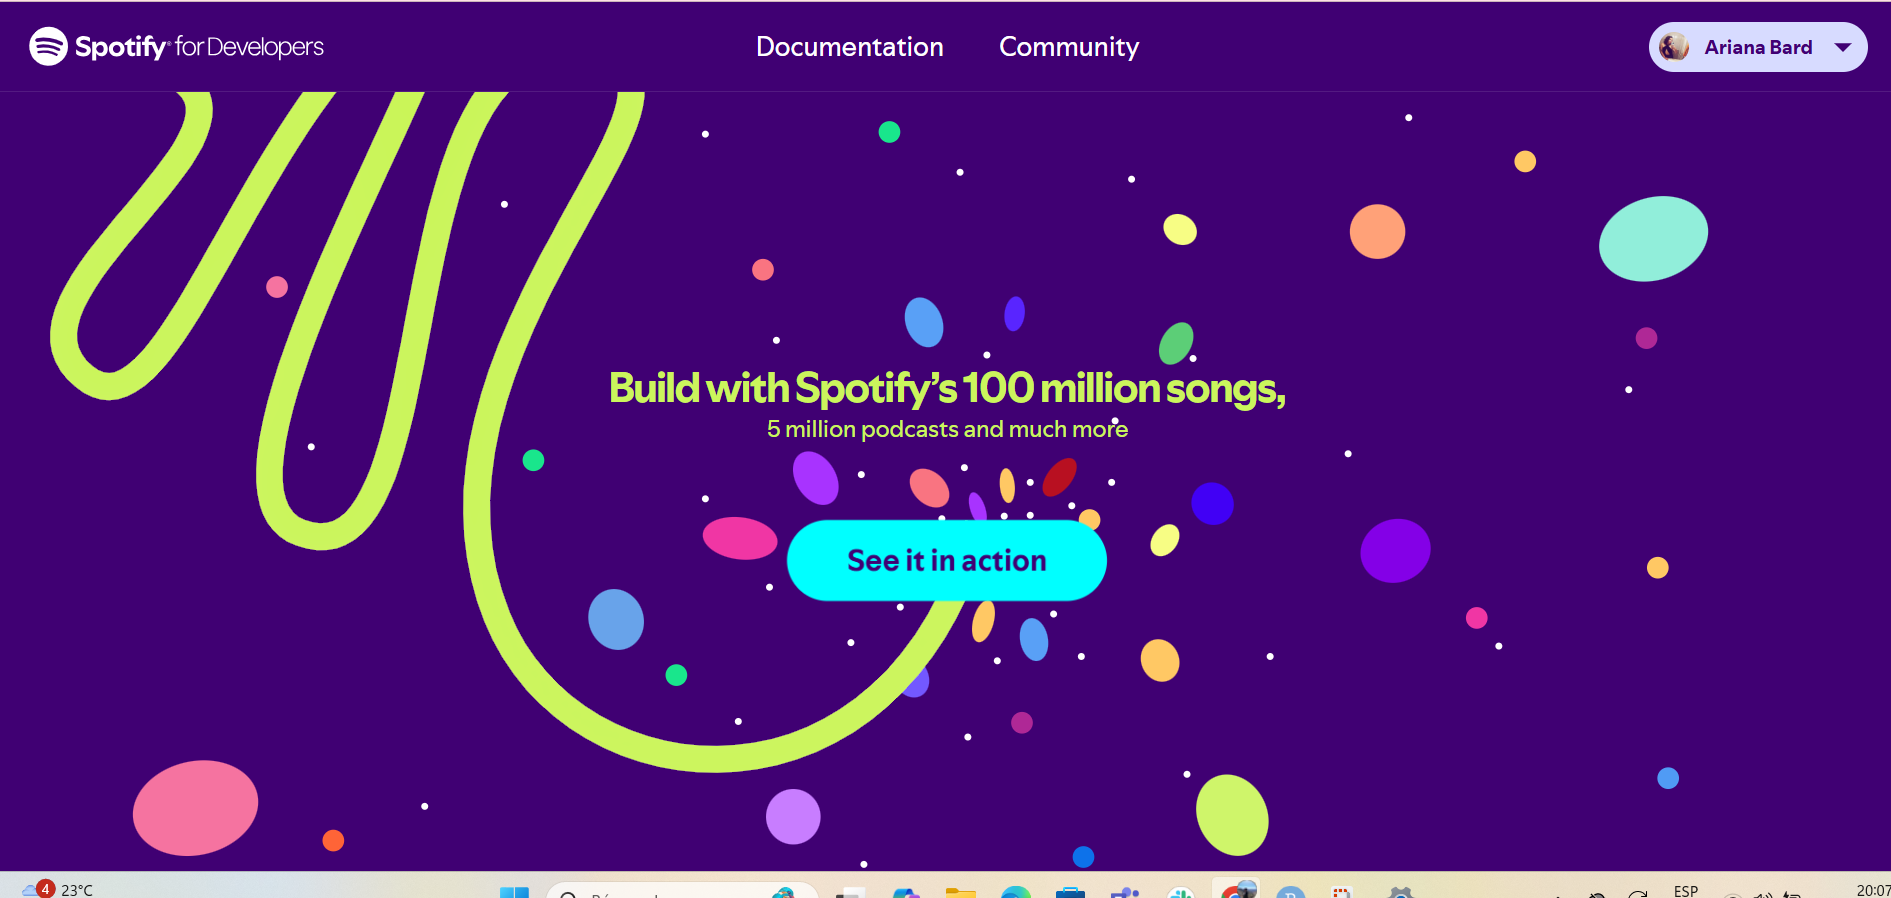
\includegraphics[keepaspectratio]{clases/presentaciones/clase_3/images/spotify_1.png}}
2) Ingresa a la solapa de
Dashboards}{ 2) Ingresa a la solapa de Dashboards}}\label{ingresa-a-la-solapa-de-dashboards}

\pandocbounded{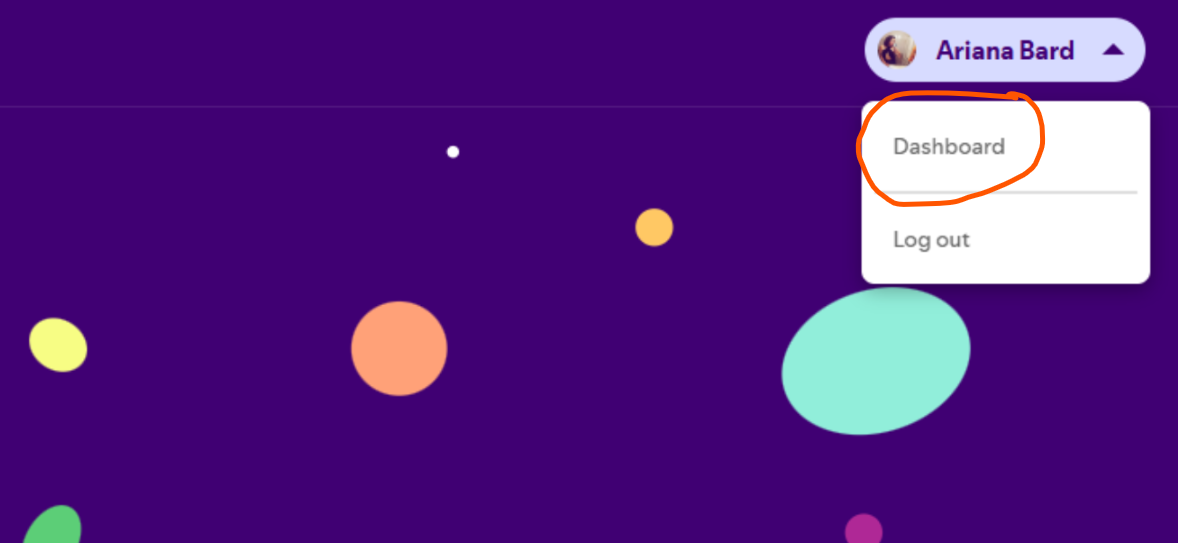
\includegraphics[keepaspectratio]{clases/presentaciones/clase_3/images/spotify_2.png}}

\subsection{3) Creá una APP}\label{creuxe1-una-app}

\pandocbounded{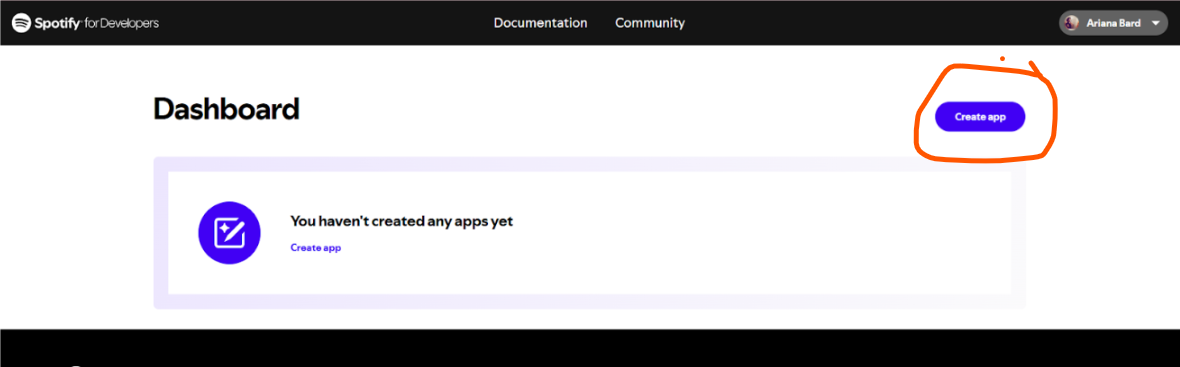
\includegraphics[keepaspectratio]{clases/presentaciones/clase_3/images/spotify_3.png}}

\subsection{4) Completá los siguientes
campos}\label{completuxe1-los-siguientes-campos}

\begin{itemize}
\tightlist
\item
  App name: UFLO clase de APIS
\item
  App description: Credenciales para clase de UFLO
\item
  Redirect URL: http://localhost:1410/
\end{itemize}

Clickear en \textbf{\texttt{create}}

\subsection{5) Copiar las credenciales y
secrets}\label{copiar-las-credenciales-y-secrets}

Los encontrarás dentro de ``settings''

\pandocbounded{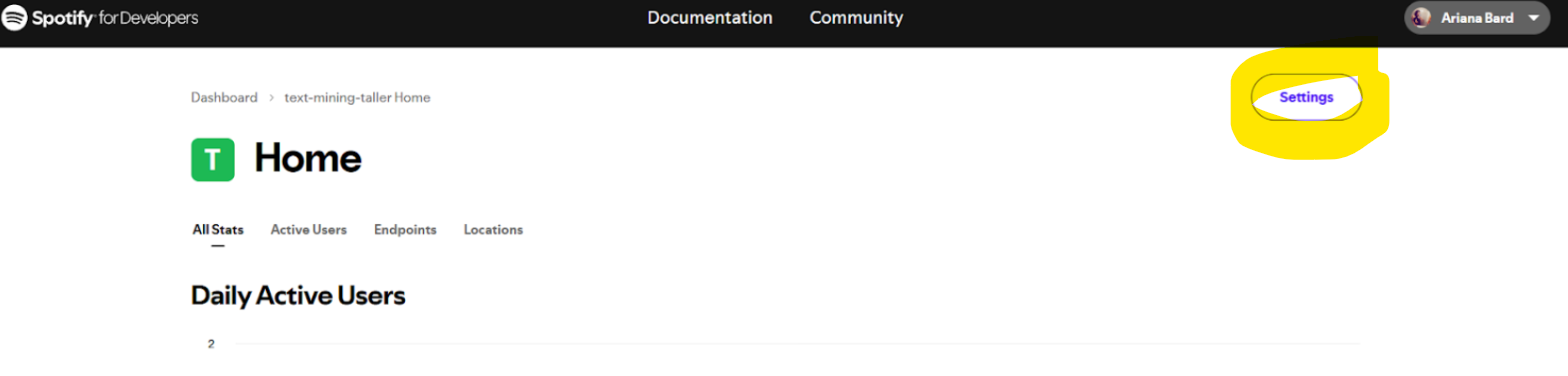
\includegraphics[keepaspectratio]{clases/presentaciones/clase_3/images/spotify_4.png}}
\pandocbounded{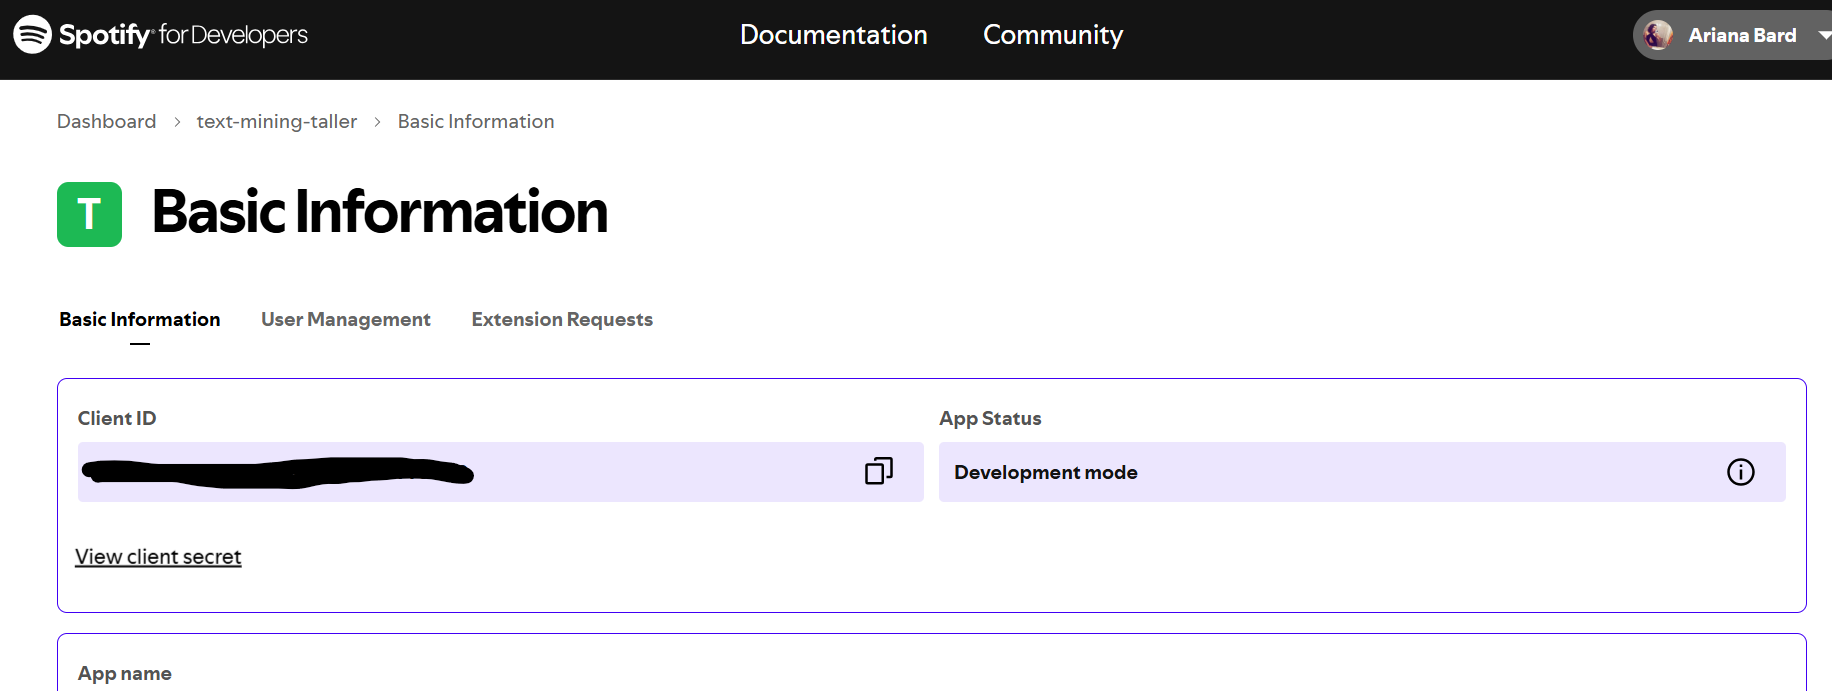
\includegraphics[keepaspectratio]{clases/presentaciones/clase_3/images/spotify_5.png}}

\chapter{C3. Presentación}\label{c3.-presentaciuxf3n}

En esta clase aprenderás a consumir APIs utilizando CURL y R. Y, a
descargar y trabajar con subtítulos de YouTube.

\chapter{C3. Actividad entregable}\label{c3.-actividad-entregable}

\section{Tarea: APIs y Análisis de Datos
Textuales}\label{tarea-apis-y-anuxe1lisis-de-datos-textuales}

\subsection{Objetivos}\label{objetivos}

\begin{enumerate}
\def\labelenumi{\arabic{enumi}.}
\item
  Descargar información de Spotify sobre los artistas más escuchados.
\item
  Consumir la API de Star Wars y descargar datos sobre los personajes.
\item
  Analizar subtítulos de un video de YouTube utilizando expresiones
  regulares.
\item
  (Opcional) Investigar y consumir otra API de tu elección.
\end{enumerate}

\subsection{Instrucciones}\label{instrucciones}

\subsubsection{Parte 1: Consumiendo datos de
Spotify}\label{parte-1-consumiendo-datos-de-spotify}

\begin{enumerate}
\def\labelenumi{\arabic{enumi}.}
\tightlist
\item
  \textbf{Conseguir tus artistas más escuchados}:
\end{enumerate}

Autentícate en la API de Spotify utilizando el paquete
\texttt{\{spotifyr\}} y descarga información sobre tus artistas más
escuchados.

Usa la función \texttt{get\_my\_top\_artists()} para obtener esta
información.

Muestra en una tabla los siguientes datos de cada artista:
\textbf{nombre}, \textbf{género}, \textbf{cantidad de oyentes
mensuales}.

\textbf{Tip}: No olvides configurar las credenciales de la API de
Spotify.

\begin{enumerate}
\def\labelenumi{\arabic{enumi}.}
\setcounter{enumi}{1}
\item
  \textbf{Análisis de álbumes}:

  \begin{itemize}
  \item
    Descarga información sobre los álbumes de uno de tus artistas más
    escuchados utilizando la función \texttt{get\_artist\_albums()}.
  \item
    Muestra en una tabla los siguientes datos: \textbf{nombre del
    álbum}, \textbf{fecha de lanzamiento}, \textbf{tipo de álbum} (ej.
    álbum, sencillo, etc.).
  \end{itemize}
\end{enumerate}

\subsubsection{Parte 2: Consumiendo datos de Star
Wars}\label{parte-2-consumiendo-datos-de-star-wars}

Utiliza la API de Star Wars (\url{https://www.swapi.tech/}) para obtener
información sobre las peliculas, los planetas y las especies

\begin{itemize}
\tightlist
\item
  Extrae los datos y muestralos en una tabla\\
\item
  Realiza una visualización con ggplot, Highcharter o librería de
  visualización que te guste
\end{itemize}

\subsubsection{Parte 3: Análisis de subtítulos de
YouTube}\label{parte-3-anuxe1lisis-de-subtuxedtulos-de-youtube}

\begin{enumerate}
\def\labelenumi{\arabic{enumi}.}
\item
  Selecciona un video de interés
\item
  \textbf{Descargar subtítulos}
\item
  Utiliza la función \texttt{get\_caption()} del paquete
  \texttt{\{youtubecaption\}}
\item
  Muestra los subtítulos descargados en una tabla.
\item
  Realiza un análisis básico sobre los subtítulos descargados. Buscá

\begin{verbatim}
 -  Palabras que se repiten con mayor frecuencia, eliminando las stopwords

 -  Frases o términos clave relacionados a X palabra utilizando expresiones regulares.
\end{verbatim}
\end{enumerate}

\subsubsection{Parte 4: (Opcional) Inspeccionar otra
API}\label{parte-4-opcional-inspeccionar-otra-api}

Explora alguna de las siguientes APIs abiertas y realiza un análisis
similar al de la API de Star Wars. Algunas son (puede ser otra)

\begin{itemize}
\item
  \href{https://pokeapi.co/}{Pokémon API} - Obtén información sobre
  Pokémon (por ejemplo, nombre, tipo, habilidades).
\item
  \href{https://thedogapi.com/}{The Dog API} - Obtén información sobre
  razas de perros, imágenes, etc.
\end{itemize}

\subsection{Entrega}\label{entrega}

\begin{enumerate}
\def\labelenumi{\arabic{enumi}.}
\tightlist
\item
  \textbf{Sube tu código y resultados en un archivo \texttt{.Rmd} o
  \texttt{.R}}.
\end{enumerate}

\begin{quote}
\textbf{No te olvides de documentar el código} explicando lo que estás
haciendo en cada paso.
\end{quote}

\part{\textbf{Clase 4. Webscrapping}}

\chapter{C4. Antes de la clase}\label{c4.-antes-de-la-clase}

\section{\texorpdfstring{\textbf{1. Instalá los
Paquetes}}{1. Instalá los Paquetes}}\label{instaluxe1-los-paquetes}

Instalá los siguientes paquetes copiando y pegando el siguiente código
en la consola de RStudio:

\begin{Shaded}
\begin{Highlighting}[]

\NormalTok{paquetes\_lista }\OtherTok{\textless{}{-}} \FunctionTok{c}\NormalTok{(}
  \StringTok{"rvest"}\NormalTok{)}

\FunctionTok{install.packages}\NormalTok{(paquetes\_lista)}
\end{Highlighting}
\end{Shaded}

\chapter{C4. Presentación}\label{c4.-presentaciuxf3n}

En esta clase aprenderás a realizar web scrapping con R

\chapter{C4. Taller práctico}\label{c4.-taller-pruxe1ctico}

\section{Tarea: Scrapear una página
web}\label{tarea-scrapear-una-puxe1gina-web}

\begin{enumerate}
\def\labelenumi{\arabic{enumi})}
\tightlist
\item
  Elegir una página web
\item
  generar un dataset a través de scrapeo con
  \href{https://rvest.tidyverse.org/}{\{rvest\}}
\end{enumerate}

\subsection{Entregable:}\label{entregable}

Archivo .R o rmd con el procesamiento

\chapter{C4. Datos personales \&
webscrapping}\label{c4.-datos-personales-webscrapping}

\begin{itemize}
\item
  Agencia de Acceso a la Información Pública (AAIP). (2023).
  \emph{Declaración conjunta sobre webscraping y protección de la
  privacidad.}
  \href{https://www.argentina.gob.ar/sites/default/files/declaracion_conjunta_aaip_datascraping.pdf}{Documento
  en línea}.
\item
  Corte Suprema de Justicia de la Nación. (2025). Nuevas tecnologías:
  Responsabilidad de los buscadores de internet.
  \href{https://sj.csjn.gov.ar/homeSJ/notas/nota/189/documento}{Documento
  en línea}
\item
  Office of the Privacy Commissioner of Canada (OPC). (2024).
  \emph{Joint statement on data scraping and the protection of privacy.}
  \href{https://www.priv.gc.ca/en/opc-news/speeches-and-statements/2024/js-dc_20241028/}{Declaración
  en línea}.
\item
  Information Commissioner's Office (ICO). (2024). \emph{ICO
  consultation series on generative AI and data protection.}
  \href{https://ico.org.uk/about-the-ico/ico-and-stakeholder-consultations/ico-consultation-series-on-generative-ai-and-data-protection/}{Consulta
  en línea}.
\end{itemize}

\part{Clase 5. Preprocesamiento: tokenización, lematización, limpieza y
eliminación de ruido textual}

\chapter{C5. Antes de la clase}\label{c5.-antes-de-la-clase}

\section{\texorpdfstring{\textbf{1. Instalá los
Paquetes}}{1. Instalá los Paquetes}}\label{instaluxe1-los-paquetes-1}

Instalá los siguientes paquetes copiando y pegando el siguiente código
en la consola de RStudio:

\begin{Shaded}
\begin{Highlighting}[]

\NormalTok{paquetes\_lista }\OtherTok{\textless{}{-}} \FunctionTok{c}\NormalTok{(}
  \StringTok{"tidytext"}\NormalTok{, }\StringTok{"stringr"}\NormalTok{, }\StringTok{"stringi"}\NormalTok{, }\StringTok{"SnowballC"}\NormalTok{, }\StringTok{"udpipe"}\NormalTok{)}

\FunctionTok{install.packages}\NormalTok{(paquetes\_lista)}
\end{Highlighting}
\end{Shaded}

\chapter{C5. Presentación}\label{c5.-presentaciuxf3n}

En esta clase aprenderás a implementar técnicas para eliminar ruido
textual (caracteres especiales, puntuación, normalización de texto) y
procesar textos en R mediante tokenización, eliminación de stopwords y
lematización.

\chapter{C5. Taller práctico}\label{c5.-taller-pruxe1ctico}

\begin{quote}
🔍 \textbf{Con el dataset o corpus de texto que vas a utilizar para tu
trabajo final}, aplicá técnicas de preprocesamiento y vectorización para
preparar el texto para su análisis.
\end{quote}

\begin{enumerate}
\def\labelenumi{\arabic{enumi}.}
\tightlist
\item
  \textbf{Aplicá los pasos de limpieza y preprocesamiento}
\item
  \textbf{Vectorizá el texto} generando una tabla de frecuencias por
  lemma o raiz.
\item
  \textbf{Visualizá los resultados}: Podés usar un gráfico de barras con
  las palabras más frecuentes o una nube de palabras que represente
  visualmente las palabras más importantes en tu corpus
\end{enumerate}

\chapter{C5. Actividad entregable}\label{c5.-actividad-entregable}

\section{📄 Diseño del trabajo final}\label{diseuxf1o-del-trabajo-final}

\begin{quote}
Esta actividad tiene como objetivo que puedas avanzar en la
planificación y delimitación de tu trabajo final, organizando sus
componentes principales.
\end{quote}

\subsection{Consigna}\label{consigna}

Presentá un documento breve que incluya los siguientes elementos:

\begin{itemize}
\tightlist
\item
  \textbf{Título tentativo del trabajo final:} Debería reflejar el tema,
  enfoque o población a estudiar.
\item
  \textbf{Objetivo general y objetivos específicos} ¿Qué te proponés
  estudiar? ¿Qué aspectos o dimensiones vas a analizar en particular?
\item
  \textbf{Pregunta de investigación}: Enunciá claramente qué
  interrogante guía el trabajo. Podés agregar una o dos subpreguntas.
\item
  \textbf{Hipótesis} (si aplica): Planteá una o más suposiciones que
  orienten el análisis (pueden ser iniciales y exploratorias).
\item
  \textbf{Metodología a utilizar} (versión preliminar): Indicá
  brevemente qué tipo de análisis pensás hacer (exploratorio,
  descriptivo, comparativo, etc.). ¿Qué técnicas de análisis de texto
  creés que vas a necesitar aplicar? (aunque aún no las hayas
  implementado)
\item
  \textbf{Descripción del corpus o conjunto de datos}: Explicá qué tipo
  de textos o documentos vas a analizar ¿De dónde provienen? ¿Cómo los
  vas a obtener? ¿Qué variables contiene el corpus? ¿Qué tipo de
  información incluye? ¿Por qué es relevante y adecuado para responder
  tu pregunta de investigación?
\item
  \textbf{Antecedentes:} ¿Existen investigaciones, artículos, papers que
  hayan trabajado sobre esta temática?
\end{itemize}

\subsection{Modalidad de entrega}\label{modalidad-de-entrega}

\begin{itemize}
\item
  Formato: PDF o Word (1 a 3 páginas aprox.)
\item
  Fecha límite: 8/05
\item
  Medio de entrega: Aula virtual
\item
  Utilizar normas APA
\end{itemize}

\part{Clase 6. POS Tagging, WSD y NER}

\chapter{C6. Antes de la clase}\label{c6.-antes-de-la-clase}

\section{\texorpdfstring{\textbf{1. Instalá los
Paquetes}}{1. Instalá los Paquetes}}\label{instaluxe1-los-paquetes-2}

Instalá los siguientes paquetes copiando y pegando el siguiente código
en la consola de RStudio:

\begin{Shaded}
\begin{Highlighting}[]

\NormalTok{paquetes\_lista }\OtherTok{\textless{}{-}} \FunctionTok{c}\NormalTok{(}
  \StringTok{"spacyr"}\NormalTok{, }\StringTok{"udpipe"}\NormalTok{, }\StringTok{"stringi"}\NormalTok{, }\StringTok{"SnowballC"}\NormalTok{, }\StringTok{"udpipe"}\NormalTok{)}

\FunctionTok{install.packages}\NormalTok{(paquetes\_lista)}

\CommentTok{\# Instala spacyr}
\FunctionTok{library}\NormalTok{(spacyr)}
\FunctionTok{spacy\_install}\NormalTok{()}

\CommentTok{\# Descarga el modelo}

\FunctionTok{spacy\_download\_langmodel}\NormalTok{(}\StringTok{"es\_dep\_news\_trf"}\NormalTok{)}
\end{Highlighting}
\end{Shaded}

\chapter{C6. Presentación}\label{c6.-presentaciuxf3n}

En esta clase exploramos \textbf{tres técnicas fundamentales del
procesamiento del lenguaje natural (NLP)} aplicadas a textos en español,
utilizando herramientas del ecosistema R: POS tagging, WDS y NER

\chapter{C6. Taller Practico}\label{c6.-taller-practico}

A partir del dataset que elijas (puede ser el corpus que estás usando
para tu trabajo final), aplicá las siguientes técnicas vistas en clase:

\begin{enumerate}
\def\labelenumi{\arabic{enumi}.}
\item
  \textbf{Cargá tu dataset en R} y realizá una exploración inicial de
  los textos.
\item
  \textbf{Aplicá POS Tagging}
\end{enumerate}

\begin{itemize}
\item
  Usá \texttt{\{udpipe\}} para etiquetar gramaticalmente las palabras.
\item
  Analizá qué categorías gramaticales predominan.
\end{itemize}

\begin{enumerate}
\def\labelenumi{\arabic{enumi}.}
\setcounter{enumi}{2}
\item
  \textbf{Aplicá Named Entity Recognition (NER)}

  \begin{itemize}
  \item
    Usá \texttt{\{spacyr\}} con un modelo en español.
  \item
    Extraé entidades de tipo PERSON, ORG y LOC.
  \item
    ¿Qué entidades aparecen con mayor frecuencia? ¿Qué revela esto del
    contenido del corpus?
  \end{itemize}
\item
  \textbf{Explorá casos de Word Sense Disambiguation (WSD)}
\end{enumerate}

\begin{verbatim}
-   Identificá al menos dos palabras polisémicas en tu corpus.

-   Mostrá en qué contextos aparecen y explicá cómo el contexto ayuda a desambiguarlas.
\end{verbatim}

\part{\textbf{Referencias}}

\chapter{Bibliografía}\label{bibliografuxeda}

\section{Text Mining}\label{text-mining}

Weiss, S. M., Indurkhya, N., \& Zhang, T. (2015). Fundamentals of
Predictive Text Mining. Capítulo 1 y 2

\section{Expresiones regulares}\label{expresiones-regulares}

Friedl, J. E. F. (2006). Mastering regular expressions: Understand your
data and be more productive (3.ª ed.). O'Reilly Media.

\chapter{📜 Licencia}\label{licencia}

Este material se publica bajo la licencia
\href{https://creativecommons.org/licenses/by-nc-sa/4.0/}{Creative
Commons Atribución-NoComercial-CompartirIgual 4.0 Internacional (CC
BY-NC-SA)}, lo que significa que:

✅ \textbf{Podés usar y modificar} el contenido siempre que menciones la
autoría.\\
🚫 \textbf{No se permite el uso comercial} del material.\\
🔄 \textbf{Si lo modificás, compartilo con la misma licencia}.

¡Disfrutalo y usalo con responsabilidad! ✨




\end{document}
